\chapter{Rendimiento en problemas de clasificación}\label{medidasRendimiento}
% \begin{quotation}
% 	\begin{small}
% 	\textit{El afán de perfección hace a algunas personas totalmente insoportables.}
% 	\end{small}
% 	\begin{flushright}Pearl S. Buck.\end{flushright}
% \end{quotation}

\section{Métricas de rendimiento}\label{2.1}
\noindent Uno de los problemas fundamentales en aprendizaje automático, (\textit{Machine
Learning},
ML), es la
clasificación en dos o más clases de un conjunto de ejemplos no conocido (conjunto de
generalización), en base al aprendizaje de un número de ejemplos
cuya	clase	si es conocida (conjunto de entrenamiento).

La evaluación del rendimiento es algo decisivo para obtener una medida del
rendimiento de un clasificador, en cuanto a los conjuntos de entrenamiento y
generalización. En ocasiones el proceso de diseño u obtención de un clasificador conlleva
una serie de etapas que implican un proceso iterativo, donde cada	iteración, puede alterar
considerablemente el clasificador que se está diseñando. Se requiere, por tanto, una
re-evaluación del clasificador en cada iteración para determinar cuál ha sido el	impacto
producido en su rendimiento, premiando, generalmente, aquellos cambios que lo han hecho
mejorar.

En la literatura existen diversas medidas para determinar el
rendimiento de un clasificador \cite{Duda2000,Caruana2004,Sokolova2009}, pero
antes de pasar a describir algunas de las más utilizadas, es conveniente definir lo que se
denomina matriz de contingencia o matriz de confusión de un clasificador.

Dado un problema de
clasificación multiclase con $Q$ clases, siendo $Q\geq2$, y $N$ patrones de entrenamiento
o generalización, la matriz de contingencia $M(g)$, de dimensión $Q\text{x}Q$, de un
clasificador $g$, está dada por:
\begin{displaymath}
\begin{tabular}{ccc}
&Clase Predicha & \\
$\mathbf{M(g)}=$ &$\left( \begin{array}{cccc}
n_{11} & n_{12} & \ldots & n_{1Q} \\
n_{21} & n_{22} & \ldots & n_{2Q} \\
\ldots & \ldots & n_{ii} & \ldots \\
n_{Q1} & n_{Q2} & \ldots & n_{QQ} \\
\end{array} \right)$ & \begin{sideways}\hspace{-0.8cm}Clase
Real\end{sideways} \\
\end{tabular}
\end{displaymath}
donde las filas indican la clase real de pertenencia y las columnas la pronosticada
por el clasificador.

Formalmente,  la matriz de confusión, $M(g)$, se puede definir como:
\begin{displaymath}
	 \mathbf{M(g)}=\left\{n_{ij};\sum_{i,j=1}^Q n_{ij}=N\right\}
\end{displaymath}
donde $n_{ij}$ representa el número de patrones asignados a la clase $i$, cuando
realmente pertenecen a la clase $j$. La diagonal corresponde a los patrones correctamente
clasificados para las $Q$ clases del problema, y los   $Q(Q-1)$	elementos fuera de la
diagonal principal corresponden a los errores de clasificación. En consecuencia, los
totales por fila indican
el número de patrones pertenecientes a cada una de las clases, y la suma de estos totales
es el tamaño de la muestra.

Si analizamos la matriz de confusión:
\begin{displaymath}
\left( \begin{array}{cccc}
n_{11} & \ldots & \ldots & n_{1Q} \\
\ldots & \ldots & n_{ij} & \ldots \\
\ldots & \ldots & \ldots & \ldots \\
n_{Q1} & \ldots & \ldots & n_{QQ} \\
\end{array}\right)
\end{displaymath}
,tenemos que:
\begin{eqnarray}
n_{i\circ} & = & \sum_{j=1}^Q n_{ij} \quad i=1,...,Q \nonumber \\
n_{\circ j} & = & \sum_{i=1}^Q n_{ij} \quad j=1,...,Q \nonumber
\end{eqnarray}
siendo $n_{i\circ}$ el total de patrones asociados la clase $i$ (suma por filas), y
$n_{\circ j}$ el número
de patrones predichos por el clasificador que se han clasificado como pertenecientes a la
clase $j$ (suma por columnas).

A partir de las expresiones anteriores, se puede deducir que $\displaystyle
\sum_{i=1}^Q n_{i\circ}=N$ y que $\displaystyle \sum_{j=1}^Q n_{\circ j}=N$. Por tanto,
las frecuencias relativas correspondientes al número de patrones de la clase $i$ sobre el
total de patrones viene dada por:
\begin{displaymath}
f_{i \circ}= \frac{n_{i \circ}}{N}
\end{displaymath}
Y la frecuencia relativa correspondiente al número de patrones que el clasificador ha
clasificado como clase $j$, con respecto al total de patrones viene dada por:
\begin{displaymath}
f_{\circ j}= \frac{n_{\circ j}}{N}
\end{displaymath}

En el caso de clasificación binaria (una clase positiva y una clase negativa), es decir,
con un valor de $Q=2$, la matriz de confusión está dada por:
\begin{displaymath}
\mathbf{M(g)} =
\left( \begin{array}{cc}
tp & fn\\
fp & tn\\
\end{array} \right)
\end{displaymath}
donde:
\begin{itemize}
\item $tp$ significa ``verdaderos positivos'', o número de elementos que son de
la clase positiva y que el clasificador ha clasificado como positivos.
\item $fn$ significa ``falsos negativos'', o número de elementos que son de la clase
positiva y que el clasificador a clasificado como negativos.
\item $fp$ significa ``falsos positivos'', o número de elementos de la clase negativa
que son clasificados como positivos.
\item $tn$ significa ``verdaderos negativos'', o número de elementos de la clase
negativa que son clasificados como negativos.
\end{itemize}

% Independientemente de que las medidas de rendimiento sean escalares, basadas en umbral,
%en
% ranking o en probabilidades, se podría diferenciar entre aquellas se utilizan solo para
% problemas binarios y aquellas que se pueden utilizar tanto en binarios como en
% multiclase.
%
% Por norma general, ninguna métrica es siempre mejor que otra a la hora de medir la
% bondad de un clasificador, ya que en muchas ocasiones depende del conjunto de
% patrones a clasificar el que una métrica nos proporcione un valor de precisión más o
% menos real sobre la capacidad que tiene un determinado clasificador. Además hay
%problemas
% en los que interesa maximizar o minimizar una medida dependiendo de nuestros
% intereses. Por ejemplo, no es lo mismo diagnosticar cáncer sobre una base de datos
% médica a un 20\% de pacientes que en realizadas no lo tienen que diagnosticar
% una carencia de cáncer a un 20\% de pacientes que en realidad si lo tienen. La
%siguientes
% secciones muestran una breve descripción de las medidas más comúnmente utilizadas.
% (¿¿¿NOS PUEDEN CRITICAR QUE NO DIGAMOS EN QUÉ SITUACIONES UTILIZAR UNA MÉTRICA Y EN
%CUÁLES
% OTRA Y PORQUÉ????)

\subsection{Métricas para problemas binarios}\label{metricasbinarios}
\noindent A continuación exponemos las métricas para problemas de clasificación binarios
que más se utilizan a la hora de obtener el rendimiento de un clasificador:
\begin{description}
\item[Precisión, C:] Efectividad global de un
clasificador o	 porcentaje	de patrones totales correctamente
clasificados. Es una medida que suele proporcionarse en tanto por
ciento.
\begin{displaymath}
C=\frac{tp+tn}{tp+fn+fp+tn}=\frac{tp+tn}{N}
\end{displaymath}
\item[Precisión positiva, P:] Porcentaje de patrones correctamente clasificados
de la clase positiva con respecto a todos los elementos que el clasificador predijo como
positivos. Dicho de otra forma sería el porcentaje de ejemplos que el clasificador ha
predicho como positivos y que realmente son positivos.
\begin{displaymath}
P=\frac{tp}{tp+fp}
\end{displaymath}
\item[Sensibilidad, TPR:] También se nombra por \textit{Recall} o
\textit{True Positive Rate} (TPR). Es el porcentaje de patrones correctamente
clasificados de la clase positiva con respecto al número total	de	elementos existentes de
esa clase, o también
se puede decir que es la efectividad del clasificador para identificar los
elementos de la clase positiva.
\begin{displaymath}
TPR=\frac{tp}{tp+fn}
\end{displaymath}
\item[Especificidad, Sp:] Porcentaje de patrones correctamente
clasificados de la
clase negativa con respecto al número total de elementos existentes de esa clase, o
también se puede decir que es la	efectividad del clasificador para identificar los
elementos de la clase negativa.
\begin{displaymath}
Sp=\frac{tn}{fp+tn}=1-FPR
\end{displaymath}
donde $FPR$ se define a continuación.
\item[Porcentaje de falsos positivos, FPR:] También se nombra por \textit{False Positive Rate}
(FPR), y se define como el porcentaje de
patrones incorrectamente clasificados de la clase negativa con respecto al número
total de elementos existentes de esa clase.
\begin{displaymath}
FPR=\frac{fp}{fp+tn}=1-Sp
\end{displaymath}
\item[\textit{Fscore}:] Es una medida que se basa en $P$ y $TPR$, y se puede
interpretar como una media ponderada de ambas. Es la relación entre los elementos
positivos y aquellos dados por el clasificador.
\begin{eqnarray}
Fscore&=&\frac{2}{\frac{1}{P}+\frac{1}{TPR}} =
2\cdot \frac{P\cdot TPR}{
	P+TPR}
% 	= \nonumber \\
% &=& \frac{(\beta^2+1)tp}{(\beta^2+1)tp+\beta^2fn+fp}
\nonumber
\end{eqnarray}
donde $\beta$ es un número real no negativo, en el caso de esta igualdad $\beta=1$.
%\item[\textit{F-measure:}] La medida F es (BUSCAR DESCRIPCION...)
%\begin{displaymath}
%F-measure=\frac{2}{\frac{1}{Precisión}+\frac{1}{Sensitivity}}
%\end{displaymath}
\item[Area bajo la curva, AUC:]
Capacidad del
clasificador para evitar una clasificación falsa, teniendo en cuenta tanto a la clase
positiva como a la negativa. Esta medida es una aproximación del área bajo una curva
ROC, y se puede ver como una transformación lineal del índice de Youden
\cite{Youden1950}. Se puede calcular de manera más precisa mediante el ``Algoritmo 2``
mostrado en \cite{Fawcett2006}. Concretamente el $AUC$ es una porción del área de un
cuadrado de lado la unidad,
estando su valor entre 0 y 1. Una aproximación al $AUC$ es la siguiente:
% Se puede demostrar que el área bajo la curva ROC es
% equivalente a la prueba de Mann-Whitney, una prueba no paramétrica aplicada a dos
%muestras
% independientes, cuyos datos han sido medidos al menos en una escala de nivel ordinal;
% también equivalente a la prueba de los signos de Wilcoxon.
% ESTA MEDIDA ESTA SACADA DEL PAPER ''a SYSTEMATIC ANALISYS OF PERFOMANCE
% FOR CLASSIFICATIONS TASK``, DICE QUE ES BINARIA Y YO HE SUPUESTO QUE SE REFIERE AL AUC
%DE
% LA CURVA ROC. POR FAVOR REVISADMELO. pONE QUE A VECES A ESTA MEDIDA SE LE LLAMA Balanced
% Accuracy (MIRAR FINAL DE LA PAGINA 429 DEL ARTICULO)
\begin{displaymath}
AUC=\frac{1}{2}\left(TPR+Sp\right)
\end{displaymath}
\item[Media geométrica, GM:] La media geométrica intenta maximizar
la precisión en las dos clases que componen un determinado problema de la forma más
balanceada posible. Aunque esta medida se puede extender para problemas multiclase su
utilización no es usual.
\begin{displaymath}
GM=\sqrt{TPR\cdot Sp}
\end{displaymath}
\end{description}

\subsection{Métricas para problemas multiclase}\label{metricasmulticlase}
\noindent A partir de la matriz de confusión multiclase mostrada en la sección \ref{2.1},
la sensibilidad de una clase $i$ en problemas multiclase, se define como, el número
de patrones correctamente predichos en esa clase con respecto al número total de patrones
de dicha clase (probabilidad de predecir correctamente un ejemplo de la clase $i$), y la
denotaremos por:
\begin{displaymath}
S_{i}=\frac{n_{ij}}{n_{i\circ}}, \qquad i=1,...,Q.
\end{displaymath}

La especificidad, $Sp$, de una clase $i$ en problemas multiclase, se define como, el número
de patrones correctamente predichos en esa clase con respecto al número total de patrones
predichos por el clasificador para esa clase. Hay que hacer notar que para problemas
binarios la
especificidad se refiere a la clase negativa, según está definida en la sección
\ref{metricasbinarios}:
\begin{displaymath}
Sp_{i}=\frac{n_{ii}}{n_{\circ j}}, \qquad j=1,...,Q.
\end{displaymath}

Teniendo en cuenta dicha matriz y las definiciones anteriores, las métricas más utilizadas
para problemas multiclase son las siguientes:
\begin{description}
	\item[Precisión, C:]  Al igual que en el caso de problemas binarios
	es el porcentaje de patrones correctamente clasificados. Es una medida que suele
	proporcionarse en tanto por ciento:
	\begin{displaymath}
	C=\left( \frac{1}{N}\right) \sum_{j=1}^Q n_{jj}
	\end{displaymath}
	Equivalentemente, $C$ puede expresarse como media ponderada de las
	sensibilidades:
	\begin{equation}\label{CenbaseS}
	C=\sum_{i=1}^Q \frac{n_{i\circ}}{N} S_{i}, \qquad i=1,...,Q\text{,}
	\end{equation}
	donde los pesos corresponden a las probabilidades "a priori" de cada clase.
	\item[Error cuadrático medio, MSE:] El error cuadrático
	medio es una medida que
	proporciona un promedio del error cometido por un clasificador entre los valores
	predichos, y los reales u observados. Los valores que puede tomar esta medida están
	entre 0 e $\infty$, y normalmente se utiliza en problemas de regresión, aunque hay
	autores que también la usan para clasificación \cite{Abbass2001,Abbass2002a}.
	\begin{displaymath}
	MSE=\left(\frac{1}{N}\right)\sum_{i=1}^N\left(\hat{Y}_{i}-Y_{i}\right)^2
	\end{displaymath}
	siendo $\hat{Y}_{i}$ la etiqueta estimada para el patrón $i$, e $Y_{i}$ la etiqueta real
	del	patrón $i$.

	En cuanto a los valores que puede tomar la variable $\hat{Y}_{i}$ y
	la variable $Y_{i}$, tanto en esta métrica como en las siguientes que se
	exponen dentro de esta sección, dependen de la interpretación que se haga de la/s
	salida/s que proporciona el clasificador que	estemos evaluando, y de los valores
	tomados como	verdaderos. Algunos ejemplos posibles de interpretación, aplicados en
	este	caso a ANNs, podrían ser los	siguientes: Una red
	neuronal	con varias salidas interpretadas de manera probabilística, donde el valor de
	cada salida indica la probabilidad de pertenencia a una clase determinada. Otra
	interpretación posible sería tener una red neuronal con una sola salida, comprendida
	entre 0 y 1, donde la pertenencia a una determinada clase se encuentra en un cierto
	rango	de esa salida. O incluso una red con varias salidas, donde cada una de ellas
	indica 0 o 1, dependiendo de si un patrón pertenece o no a una clase determinada. Por tanto,
	habrá
	que adaptar los valores $\hat{Y}_{i}$ y los valores $\hat{Y}_{i}$, de forma que se
	pueda aplicar la correspondiente métrica.
	\item[Raíz del error cuadrático medio, RMSE:] La raíz
	cuadrada	del error cuadrático
	medio, también proporciona un promedio del error cometido por un clasificador. Sus
	valores también están entre 0 e $\infty$.
	\begin{displaymath}
	RMSE=\sqrt{\left(\frac{1}{N}\right)\sum_{i=1}^N\left(\hat{Y}_{i}
	-Y_{i}\right)^2}
	\end{displaymath}
	\item[Entropía cruzada, E:] La entropía cruzada, es una función
	de error basada en
	las probabilidades de pertenencia de cada uno de los patrones de un conjunto de datos a
	cada una de las clases que componen un determinado problema. Los valores que puede
	tomar esta medida están	entre 0 e $\infty$.
	\begin{displaymath}
	E=-\left(\frac{1}{N}\right)\sum_{n=1}^N\sum_{l=1}^Qy_{n}^{(l)}\log
	g_{l}^{}(\mathbf{x}_{n})
	\end{displaymath}
	donde $y_{n}^{(l)}$ es igual a 1 si el patrón $n$ pertenece a la clase $l$, y 0 en caso
	contrario, y donde  $\displaystyle g_{l}^{}(\mathbf{x}_{n})$ es la probabilidad de que
	el patrón $n$ 	pertenezca a la clase $l$.
% 	\item[\textit{SEP (Standar Error Prediction):}] El error estándar de predicción es
% 	es una medida adimensional y se define como la	desviación típica de las diferencias
% 	entre los valores predichos y los valores reales. Al igual que el \textit{MSE} suele
% 	utilizarse en problemas de regresión.
% 	\begin{displaymath}
% 	SEP=\left( \frac{100}{\overline{Predicho}}\right)
% 	\sqrt{\left(\frac{1}{N}\right)\sum_{i=1}^N\left(Predicho(g)-Verdadero(g)\right)^2}
% 	\end{displaymath}
% 	donde $\overline{Predicho}$ es el valor medio de todas las salidas predichas por el
% 	clasificador.
% 	\item[Coeficiente de información mutua, IC:]
% 	Define la información aportada
% 	por una variable aleatoria sobre otra, o lo que es lo mismo, cuánto reduce la
% 	incertidumbre sobre una variable el conocimiento de la otra \cite{Baldi2000}. La
% 	expresión que se muestra a continuación se obtiene asumiendo que $\displaystyle
% 	H(X)=-\sum_{i}^{Q}X_{i}\log X_{i}$,
% 	y que $\displaystyle f=\frac{n_{i\circ}}{N}$, $\displaystyle k=\frac{n_{\circ j}}{N}$ y
% 	$\displaystyle n=\frac{n_{ij}}{N}$:
% 	\begin{eqnarray}
% 	IC&=&\frac{H(f)+H(k)-H(N)}{H(f)}=\nonumber \\
% 	&=&\frac{-\sum_{i=1}^Q\left(\frac{n_{i\circ}}{N}\log
% 	\frac{n_{i\circ}}{N}\right) -\sum_{i=1}^Q \left( \frac{n_{\circ j}}{N}\log
% 	\frac{n_{\circ j}}{N}\right) +\sum_{i,j=1}^Q \left( \frac{n_{ij}}{N}\log
% 	\frac{n_{ij}}{N}\right)}{-\sum_{i=1}^Q\left( \frac{n_{i\circ}}{N}\log
% 	\frac{n_{i\circ}}{N}\right)} \nonumber
% 	\end{eqnarray}
	\item[\textit{Generalized Squared Correlation}, GC$^{2}$:] La correlación
	cuadrática generalizada se puede considerar como una generalización para problemas
	multiclase del coeficiente de correlación de Matthews \cite{Matthew1975} para dos
	clases.
	\begin{displaymath}
	GC^2=\frac{1}{N\left(Q-1\right)}\sum_{i,j=1}^Q\frac{\left(
	n_{ij}-e_{ij}\right)^2}{e_{ij}}
	\end{displaymath}
	donde $\displaystyle e_{ij}=\frac{n_{i\circ}n_{\circ j}}{N}$	es el número esperado de
patrones en
	la posición	$ij$ de la matriz de confusión, teniendo como hipótesis que las asignaciones
	y	las	predicciones son independientes.
	\item[\textit{Macro-Average}, MAVG:] La macro-media se define como la media de las
	sensibilidades de cada clase, sin considerar la desviación típica. Da la misma
	importancia o peso a cada una de las clases de un problema.
	\begin{displaymath}
	MAVG=\frac{1}{Q}\sum_{i=1}^Q S_{i}
	\end{displaymath}
\end{description}
\newpage
\section{Curvas ROC}\label{curvasROC}
\noindent Cabe comentar por separado una de las técnicas más usadas habitualmente para
la comparación del rendimiento mostrado por dos o más clasificadores binarios, las
llamadas curvas
ROC \cite{Fawcett2006}. Dichas curvas son	una alternativa al
uso de la		precisión	y sus		problemas derivados \cite{Provost1997,Provost1998}, y
es	una buena	técnica para		comprobar si un
clasificador es mejor que	otro	en	términos de	la clase	minoritaria. Las curvas ROC son
gráficas en dos dimensiones, en la que se representan los errores de clasificación de la
clase negativa o $FPR$ en el eje horizontal, y la precisión de la clase positiva o
$TPR$ en el eje vertical. Las curvas ROC muestran
toda la información relacionada con el rendimiento de un clasificador, y permiten una
rápida visualización del tipo de relación entre los rendimientos de varios
clasificadores. El análisis de la curva ROC, o simplemente análisis ROC, proporciona
información para seleccionar los modelos posiblemente óptimos, y es también independiente
de la distribución de las clases en la población. El análisis ROC se relaciona de forma
directa con el análisis de coste-beneficio en toma de decisiones en diagnóstico médico.

Dentro de una gráfica ROC, un clasificador domina a otro mientras más arriba y más a la
izquierda se encuentre (ver figura \ref{ejemploROC}). El mejor método posible de
predicción se situaría en un punto en la esquina superior izquierda, o coordenada $(0,1)$
del plano ROC, representando un 100\% de sensibilidad (ningún falso negativo) y un 100\%  de
especificidad (ningún falso positivo). Este punto $(0,1)$ se denomina
clasificación perfecta. Por el contrario, una clasificación totalmente aleatoria daría
un punto a lo largo de la línea diagonal (línea de no-discriminación),
desde el extremo inferior izquierdo hasta el extremo superior derecho.

\begin{figure*}[htb]
\centering
\subfloat[Curva ROC]{\label{ejemploROC1}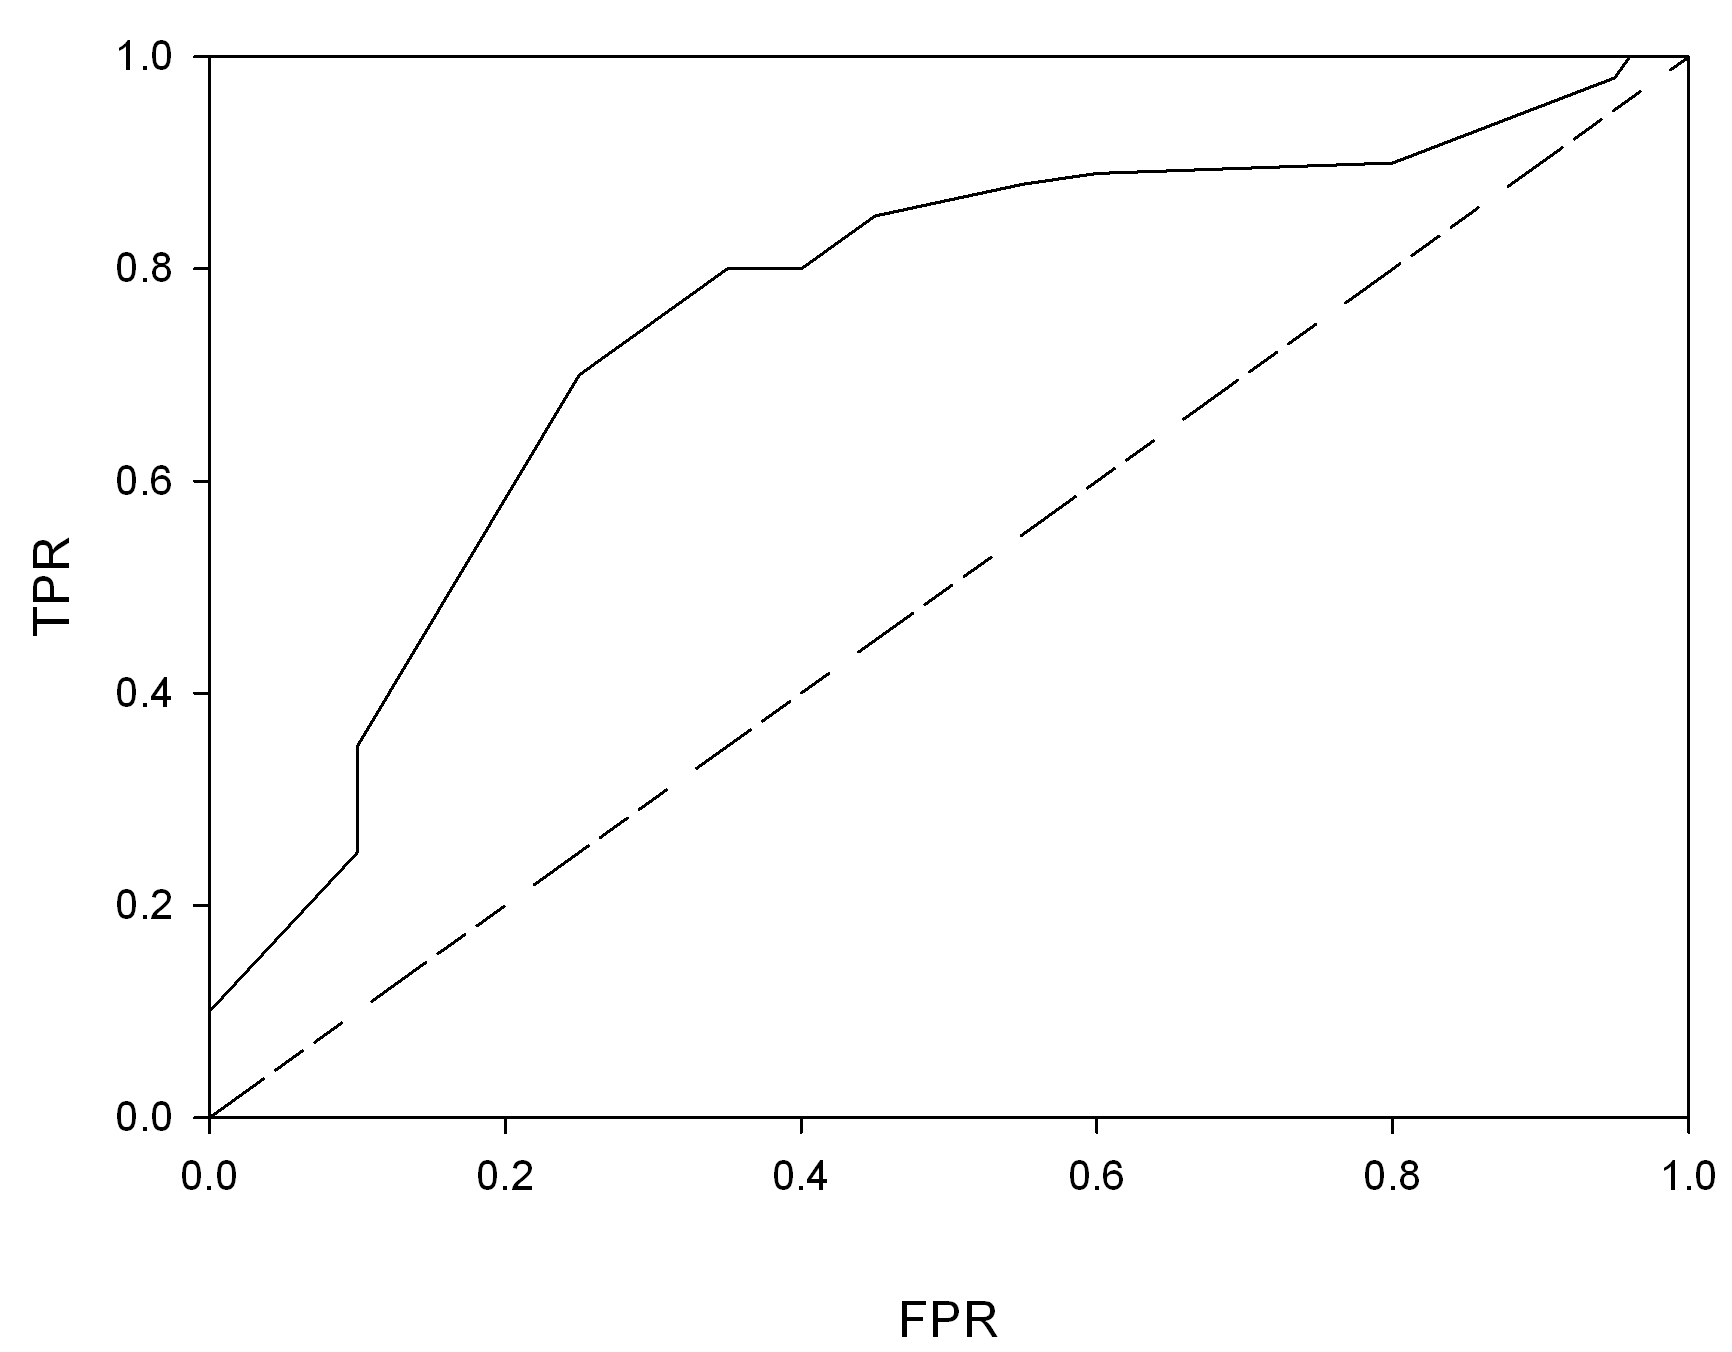
\includegraphics[width=.50
\textwidth]{figuras/curvaROC.jpg}}
\subfloat[Clasificador aleatorio]{\label{ejemploROC4}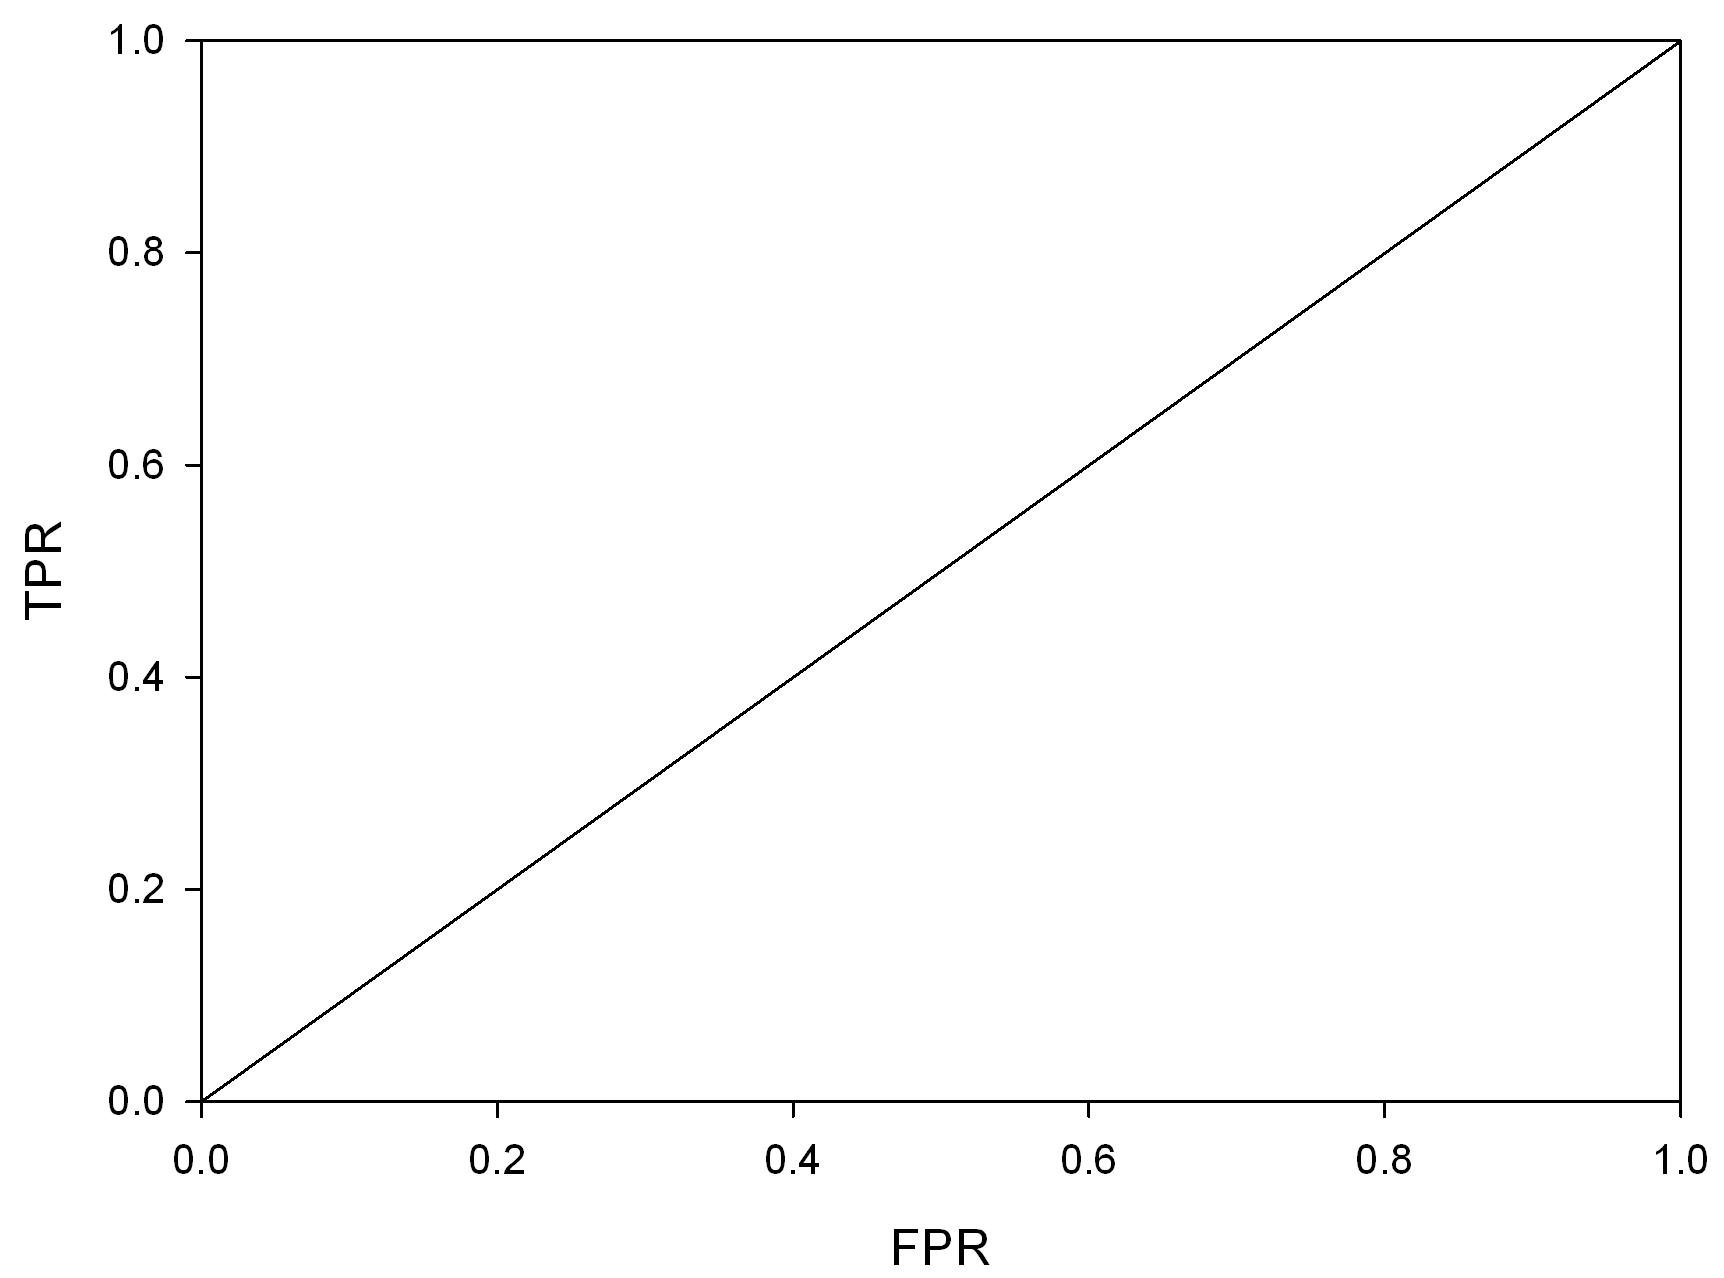
\includegraphics[width=.50
\textwidth]{figuras/curvaROCrealidad.jpg}} \\
\subfloat[Buen clasificador (alto
\textit{TPR} y bajo \textit{FPR})]{\label{ejemploROC2}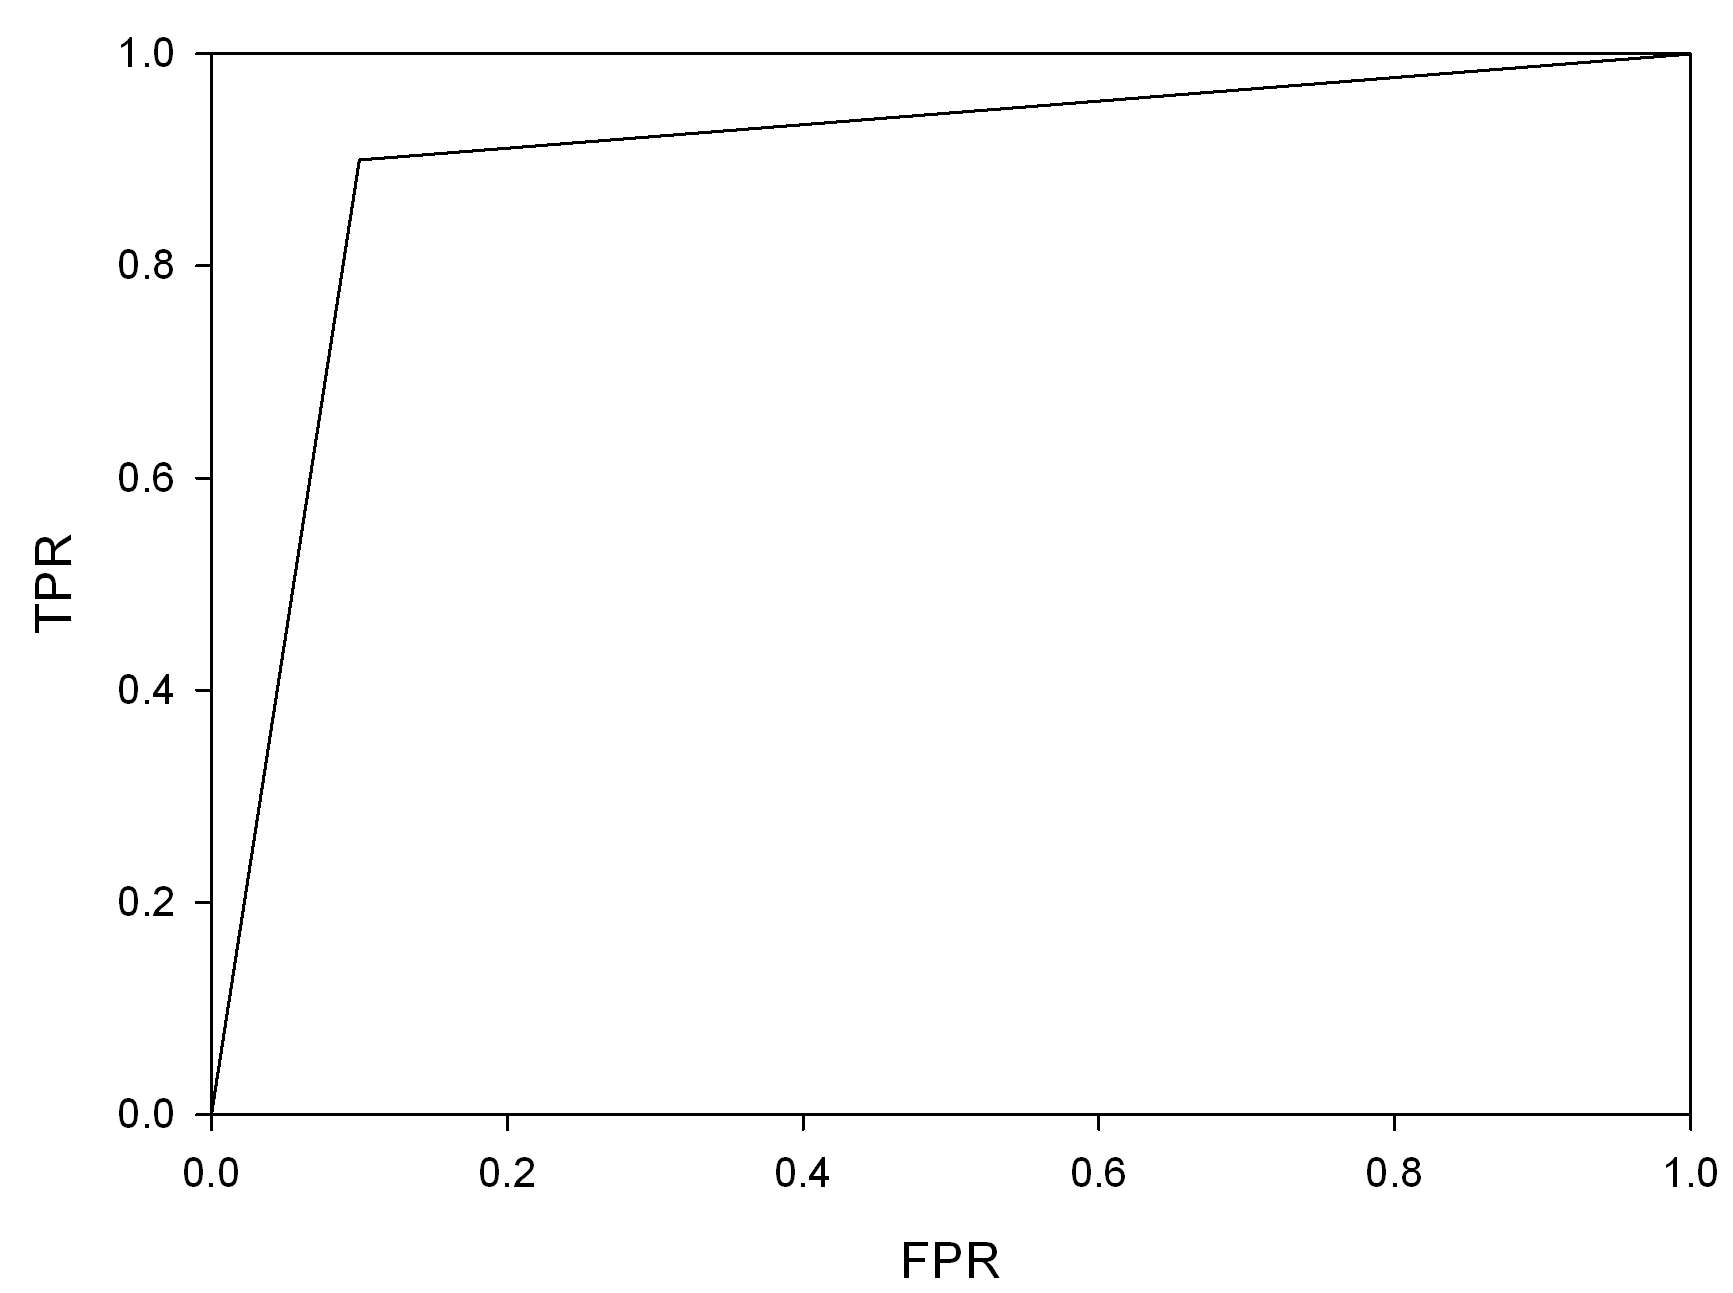
\includegraphics[width=.50
\textwidth]{figuras/curvaROCbueno.jpg}}
\subfloat[Mal clasificador, (bajo
\textit{TPR} y alto \textit{FPR})]{\label{ejemploROC3}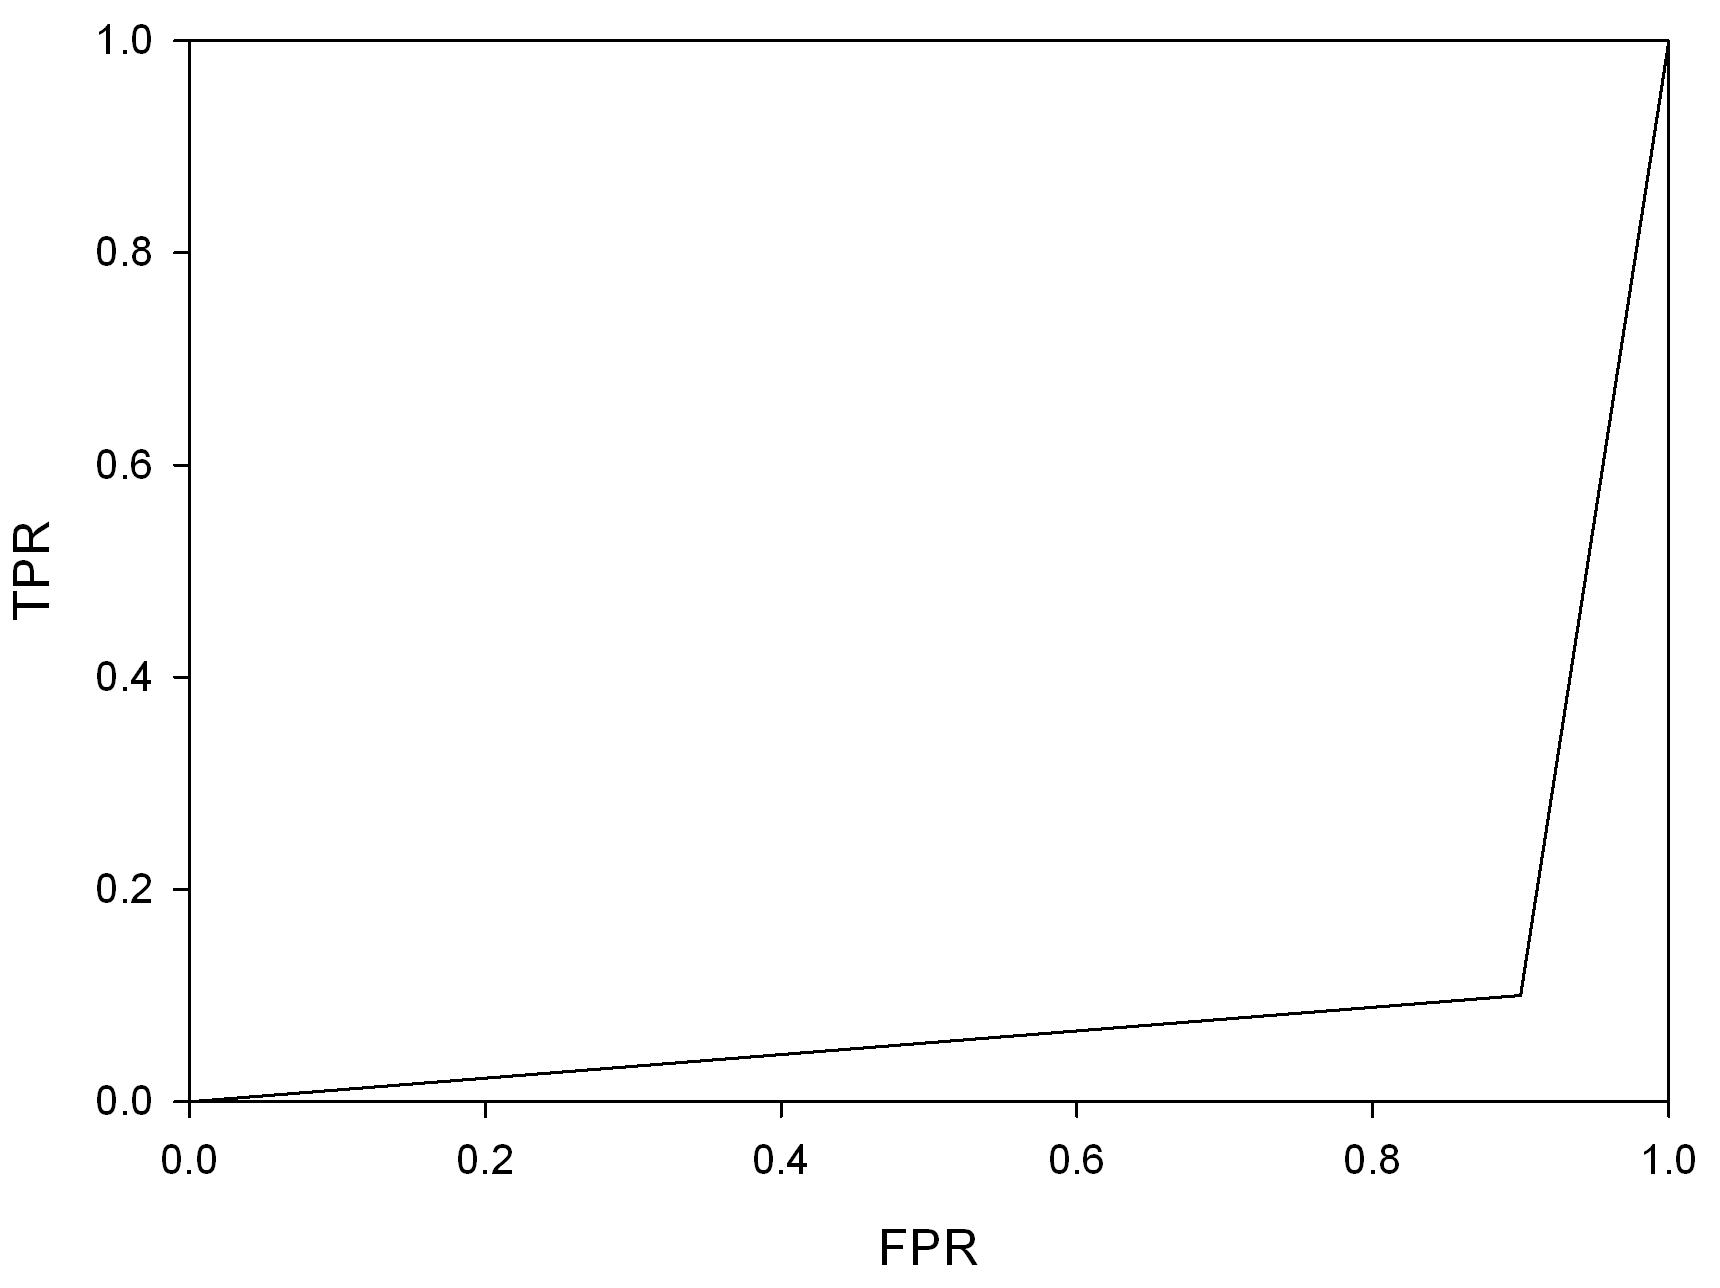
\includegraphics[width=.50
\textwidth]{figuras/curvaROCmalo.jpg}}

\caption{Ejemplos de curvas ROC}
\label{ejemploROC}
\end{figure*}

La extensión de las curvas ROC para dos clases a problemas multiclase
es interesante, ya que conferiría los beneficios del análisis ROC a más
problemas en reconocimiento de patrones. Se han realizado multitud de aproximaciones,
aunque actualmente no hay ningún análisis sobre
este tema que esté completamente consolidado \cite{Lachiche2003}. En \cite{Everson2006}, se
considera un problema de optimización	multi-objetivo donde el objetivo es minimizar
simultáneamente los $Q(Q-1)$ errores de	clasificación dados por los valores no
pertenecientes a la diagonal principal de la matriz de	confusión, donde el error se
define por $\displaystyle \frac{n_{ij}}{n_{i\circ}}$, para $i=1,2,...,Q$ y $j\neq i$. De
esta forma, el coste computacional crece en función del número de	clases. En
\cite{Langrebe2008}, se propone un algoritmo que a partir de la matriz de confusión
de un clasificador identifica las clases independientes y grupos de clases que
interactúan entre sí, permitiendo la descomposición de la matriz en un curva ROC con un
número bajo de grupos dimensionales. Esto reduce la complejidad computacional
considerablemente. La hiper-superficie ROC descompuesta se puede tratar como en el
caso ideal (dos clases), permitiendo realizar aproximaciones coste-beneficio y la
aproximación de Neyman-Pearson \cite{Edwards2004}, así como el volumen bajo la curva,
AUC. Otra manera de trabajar con problemas multi-clase es mediante el uso del
volumen sobre la superficie ROC (\textit{Volume under Surface}, VUS) \cite{Dreiseitl2007}
con curvas en 3-D \cite{Sahiner2008,He2008}. Así por ejemplo, en \cite{Mossman1999}, el
concepto de curvas ROC se extiende a cuestiones de diagnóstico médico con tres
posibles alternativas; se dibuja una superficie ROC en tres dimensiones para una
tarea de decisión tridimensional, añadiendo el VUS sobre la superficie ROC. De esta
manera, el VUS resume la precisión global del modelo,
similar al AUC de una curva ROC hecho sobre una tarea de
clasificación con dos	alternativas. La obtención de información en los puntos de la
superficie se puede	calcular de la misma forma que para curvas ROC bidimensionales, así,
se pueden comparar tres tipos de curvas ROC bidimensionales, en función de la información
de cada superficie.
% Otra aproximación en problemas multiclase consiste en considerar los
% errores de clasificación de cada una de las clases, es decir, el porcentaje de falsos
% positivos para
% cada clase, definidos por los elementos exteriores a la diagonal principal de la matriz
% de
% confusión, en lugar de los errores de clasificación de cada una de las otras clases.
% Así,
% el problema queda reducido a la minimización de los $Q$ objetivos definidos por
% \begin{displaymath}
% \frac {\sum_{i\neq j}^{Q}n_{ij}}{n_{i\circ}}, \quad i=1,,2,...,Q.
% \end{displaymath}

De forma general, en el caso de utilizar MOEAs para la resolución de problemas multiclase
mediante aproximaciones ROC, se deben tener presentes algunos inconvenientes:
\begin{enumerate}
	\item La dimensión de los frentes de Pareto crece junto con el número de clases del
	problema, haciendo extremadamente difícil encontrar soluciones que dominen al resto.
	Esto es debido a que mientras más crezca el espacio
	de objetivos, más complicado es que una solución sea mejor que otra en al menos uno
	de los objetivos e igual en los demás, según la definición de no-dominancia
	\cite{Coello2007}.
	\item El coste computacional a la hora de obtener modelos de red también aumenta
	considerablemente, ya que el número de comparaciones y operaciones a realizar para
	obtener individuos no dominados crece exponencialmente, cuadráticamente o
	linealmente con el número de clases.
	\item Los	sucesivos	frentes de Pareto que conforman la población de
	soluciones tendrán	cada vez menos individuos, a medida que aumente el número de
	objetivos ($Q(Q-1)$ errores de	clasificación) a optimizar en el problema. Esto
	hace que una de las principales	ventajas de los MOEAs, que es el proporcionar al
	experto un amplio abanico de	soluciones igualmente válidas, no se aproveche.
	\item Trabajar con más de dos objetivos tiene la desventaja de que el número
	de dimensiones de las representaciones gráficas aumenta, y por tanto sea más
	difícil su análisis e interpretación.
	\end{enumerate}

% Para reducir estos inconvenientes, normalmente lo que se intenta es hacer una
% aproximación
% trabajando solo con los errores de clasificación
% para cada clase, es decir, los falsos positivos en lugar del error de clasificación en
% cada una de	las otras clases (definido por los elementos que hay fuera de la diagonal
% principal	de la matriz de confusión). Esta propuesta reduce la dimensión del
% problema desde el	punto de vista del número de objetivos, sin embargo, esta
% proyección solo suele ser efectiva para problemas de tres clases.

\section{Mínima Sensibilidad-Precisión ($MS,C$)}\label{ms-c}
\noindent Teniendo en cuenta las definiciones dadas en la sección
\ref{metricasmulticlase}, se puede definir la Mínima Sensibilidad, $MS$, de un
clasificador $g$, como el mínimo valor de las sensibilidades de cada una de las clases
de un problema:
\begin{displaymath}
MS=min\left\lbrace S_{i};i=1,...,Q\right\rbrace
\end{displaymath}

La principal ventaja de las medidas de rendimiento mencionadas en la sección \ref{2.1}
es su simplicidad, ya que resumen o recogen de manera más o menos precisa, en un solo
valor numérico, el rendimiento de un clasificador. Sin embargo, esta simplicidad es a la
vez un punto débil, ya que un mismo valor proporcionado por uno de esos indicadores puede
representar diferentes situaciones. Si se asume que todos los errores de clasificación son
igualmente costosos, y que no hay preferencia ni penalización por un determinado conjunto
de patrones, un buen clasificador debería obtener un alto nivel de precisión global, así
como un aceptable nivel de precisión para cada clase. La precisión no puede capturar todos
los aspectos de
comportamiento	de dos clasificadores diferentes \cite{Provost1997,Provost1998}, y no es
suficiente, en algunos casos, para	determinar la calidad de un clasificador.

En esta tesis proponemos una medida de rendimiento bidimensional, de manera que pueda estar
en un punto intermedio entre las medidas unidimensionales como $C$, y las
multidimensionales dadas por los errores de clasificación, definidos por los elementos
exteriores a la diagonal principal de la matriz de confusión. Así, se intentan evitar los
problemas y limitaciones de las medidas unidimensionales, sin sufrir los
problemas relacionados con las medidas en $Q$ dimensiones (inconvenientes comentados
anteriormente de las aproximaciones
basadas en los $Q(Q-1)$ porcentajes de mala clasificación). Consideremos por tanto, como
compromiso entre ambas posibilidades, las medidas $(MS,C)$ como medidas que expresan dos
características asociadas con un clasificador: el rendimiento global, $C$, y el porcentaje
de aciertos de la clase peor clasificada, $MS$.

La selección de $MS$ como una medida complementaria de $C$ se puede justificar
considerando que la ecuación (\ref{CenbaseS}) es la media ponderada de las
sensibilidades de cada una de las $Q$ clases. Desde un punto de vista estadístico, $C$ es
una medida buena y representativa del conjunto de las sensibilidades, si éstas son lo
suficientemente homogéneas, aunque no será una medida representativa si las sensibilidades
están muy dispersas. Teniendo en cuenta este hecho, una medida complementaria de $C$ se
podría obtener considerando alguna medida que minimizase dicha dispersión, por ejemplo, el
rango $R=max\{S_{i}\}-min\{S_{i}\}$ podría ser una posible elección. Esta minimización
se puede	alcanzar si se minimiza $max\{S_{i}\}$ o se maximiza $min\{S_{i}\}$. La primera
opción no es apropiada, ya que $C$ aumenta si las sensibilidades aumentan,
por tanto la segunda alternativa es la más apropiada. De esta forma $MS=min\{S_{i}\}$, se
puede	considerar como la medida complementaria de $C$, cuyo valor hay que maximizar.

\subsection{Ejemplos}
La consideración simultanea de $MS$ y $C$ puede ayudar a clarificar los
errores y confusión que generan por si solas las medidas unidimensionales, veamos algunos
ejemplos y contra-ejemplos sobre ello:

\textbf{Ejemplo 1 (inadecuación de $C$):} Consideremos un problema de
clasificación con tres clases, y las matrices de confusión, $A$ y $B$, asociadas a dos
clasificadores, $f$ y $g$.
\begin{equation} \nonumber
A=\left( \begin{array}[c]{ccc}
60 & 0 & 0\\
0 & 30 & 0\\
5 & 4 & 1
\end{array}\right) \quad
B=\left( \begin{array}[c]{ccc}
57 & 3 & 0\\
0 & 30 & 0\\
5 & 1 & 4
\end{array}\right)
\end{equation}
Ambos clasificadores tienen la misma precisión $\displaystyle C=\frac{91}{100}=0.91$. Sin
embargo, el rendimiento en las clases es muy diferente. La $MS$ del clasificador
$f$ es $\displaystyle S_{f}= min\left\lbrace 1,1,0.1\right\rbrace=0.1 $, mientras que la
$MS$ de $g$ es $\displaystyle S_{G}= min\left\lbrace 0.95,1,0.4\right\rbrace=0.4 $. Este
ejemplo muestra claramente que la precisión no es una medida óptima para evaluar la
calidad de un clasificador, ya que no tiene en cuenta la clasificación individual de las
clases, sino un resultado general.

En problemas altamente desbalanceados, por norma general, hay un error no uniforme a
favor de la clase minoritaria (a menudo la clase de mayor interés). De esta manera, los
clasificadores que optimizan la precisión son cuestionables, en cuanto a que raramente
predicen de manera adecuada la clase minoritaria.

\textbf{Contraejemplo 1:} La $MS$ de un clasificador $f$ es $\displaystyle
MS_{f}=Min\left\lbrace 1,1,0.1\right\rbrace=0.1$, mientras que la de un clasificador
$g$ es $\displaystyle MS_{g}=Min\left\lbrace 0.95,1,0.4\right\rbrace=0.4$. En la figura
\ref{marianoejemplo1} se pueden ver los clasificadores $f$ y $g$ dentro del plano
$(MS,C)$. Claramente se puede considerar el clasificador $g$ mejor que el $f$.

\begin{figure*}[!htb]
\centering
\subfloat[]{\label{marianoejemplo1}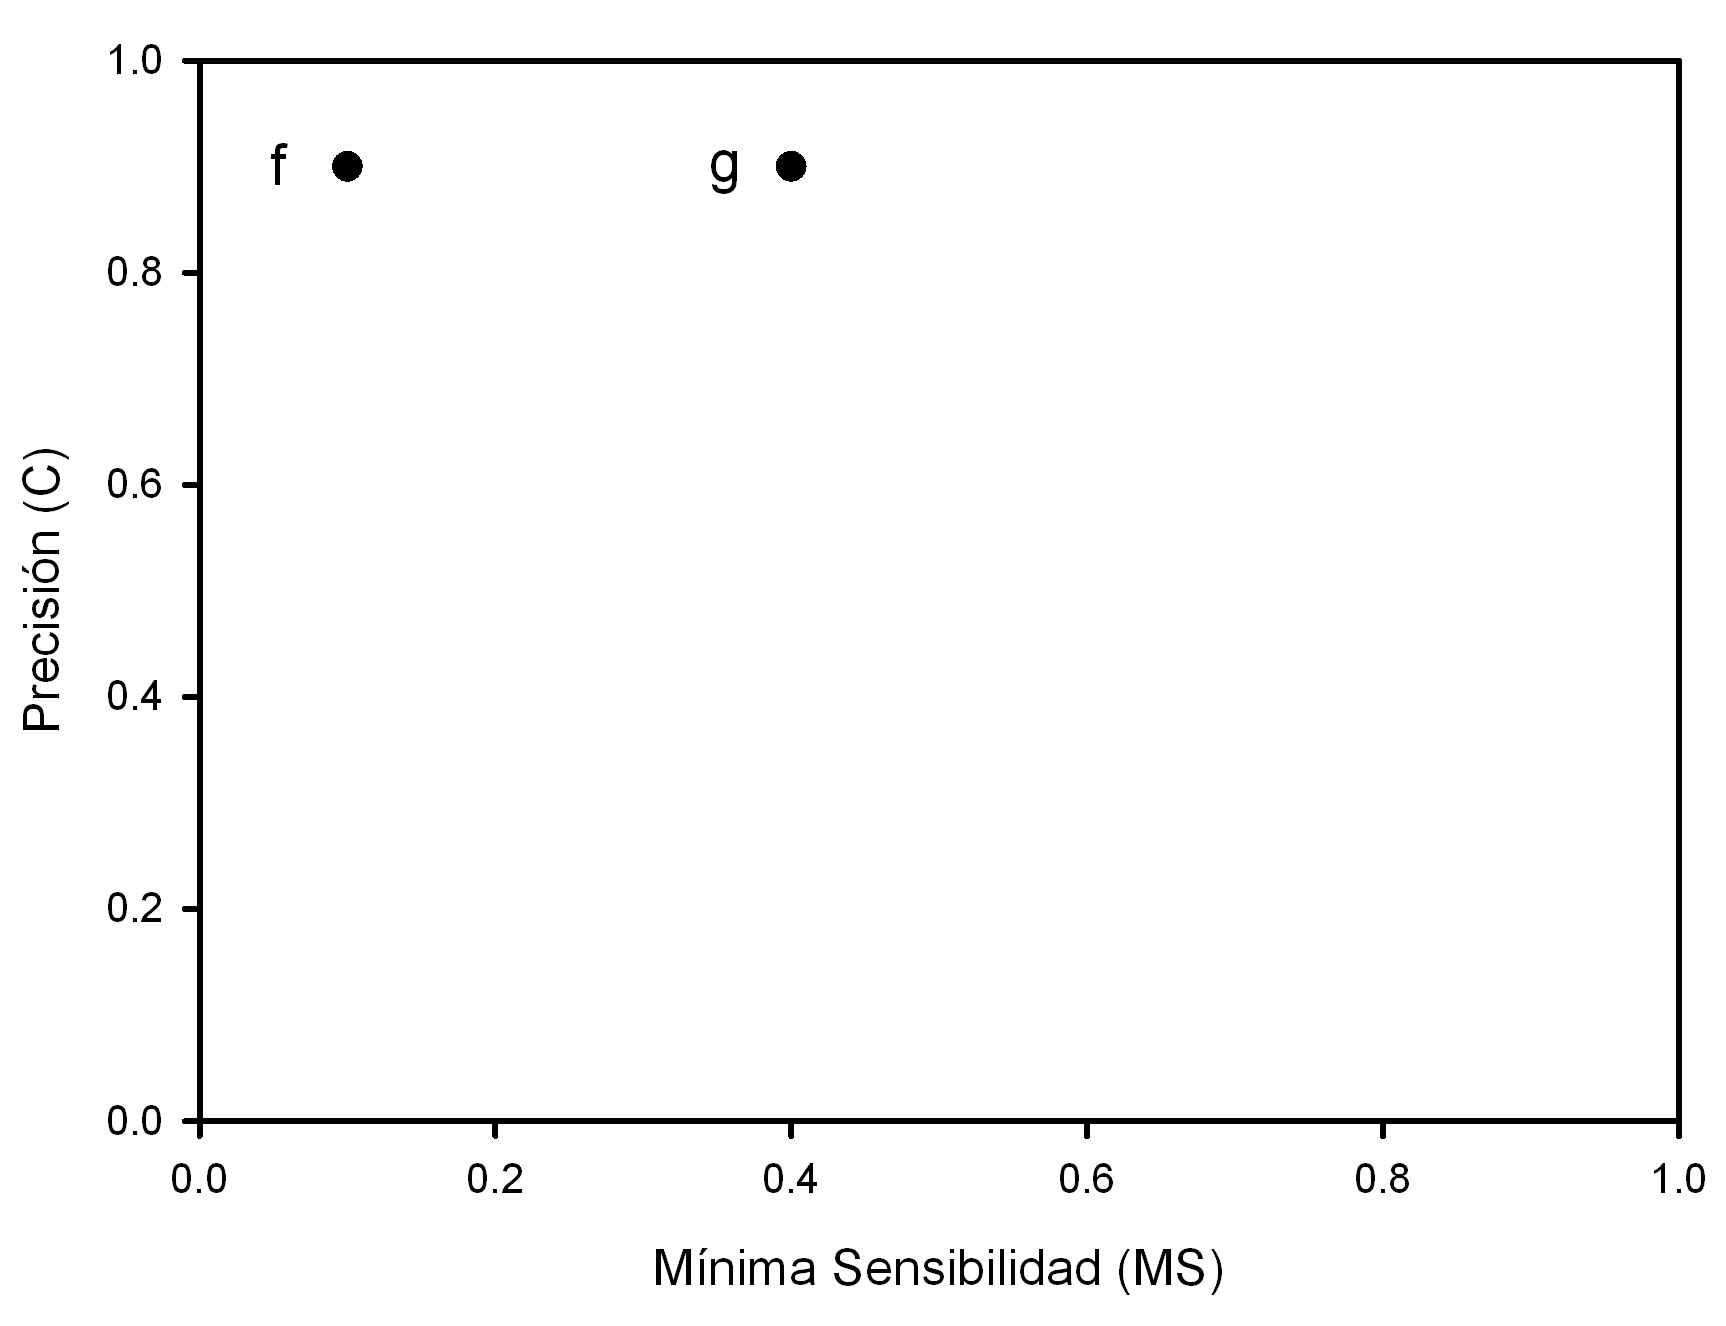
\includegraphics[width=.50
\textwidth]{figuras/articuloMarianoFigure2.jpg}}
\subfloat[]{\label{marianoejemplo3}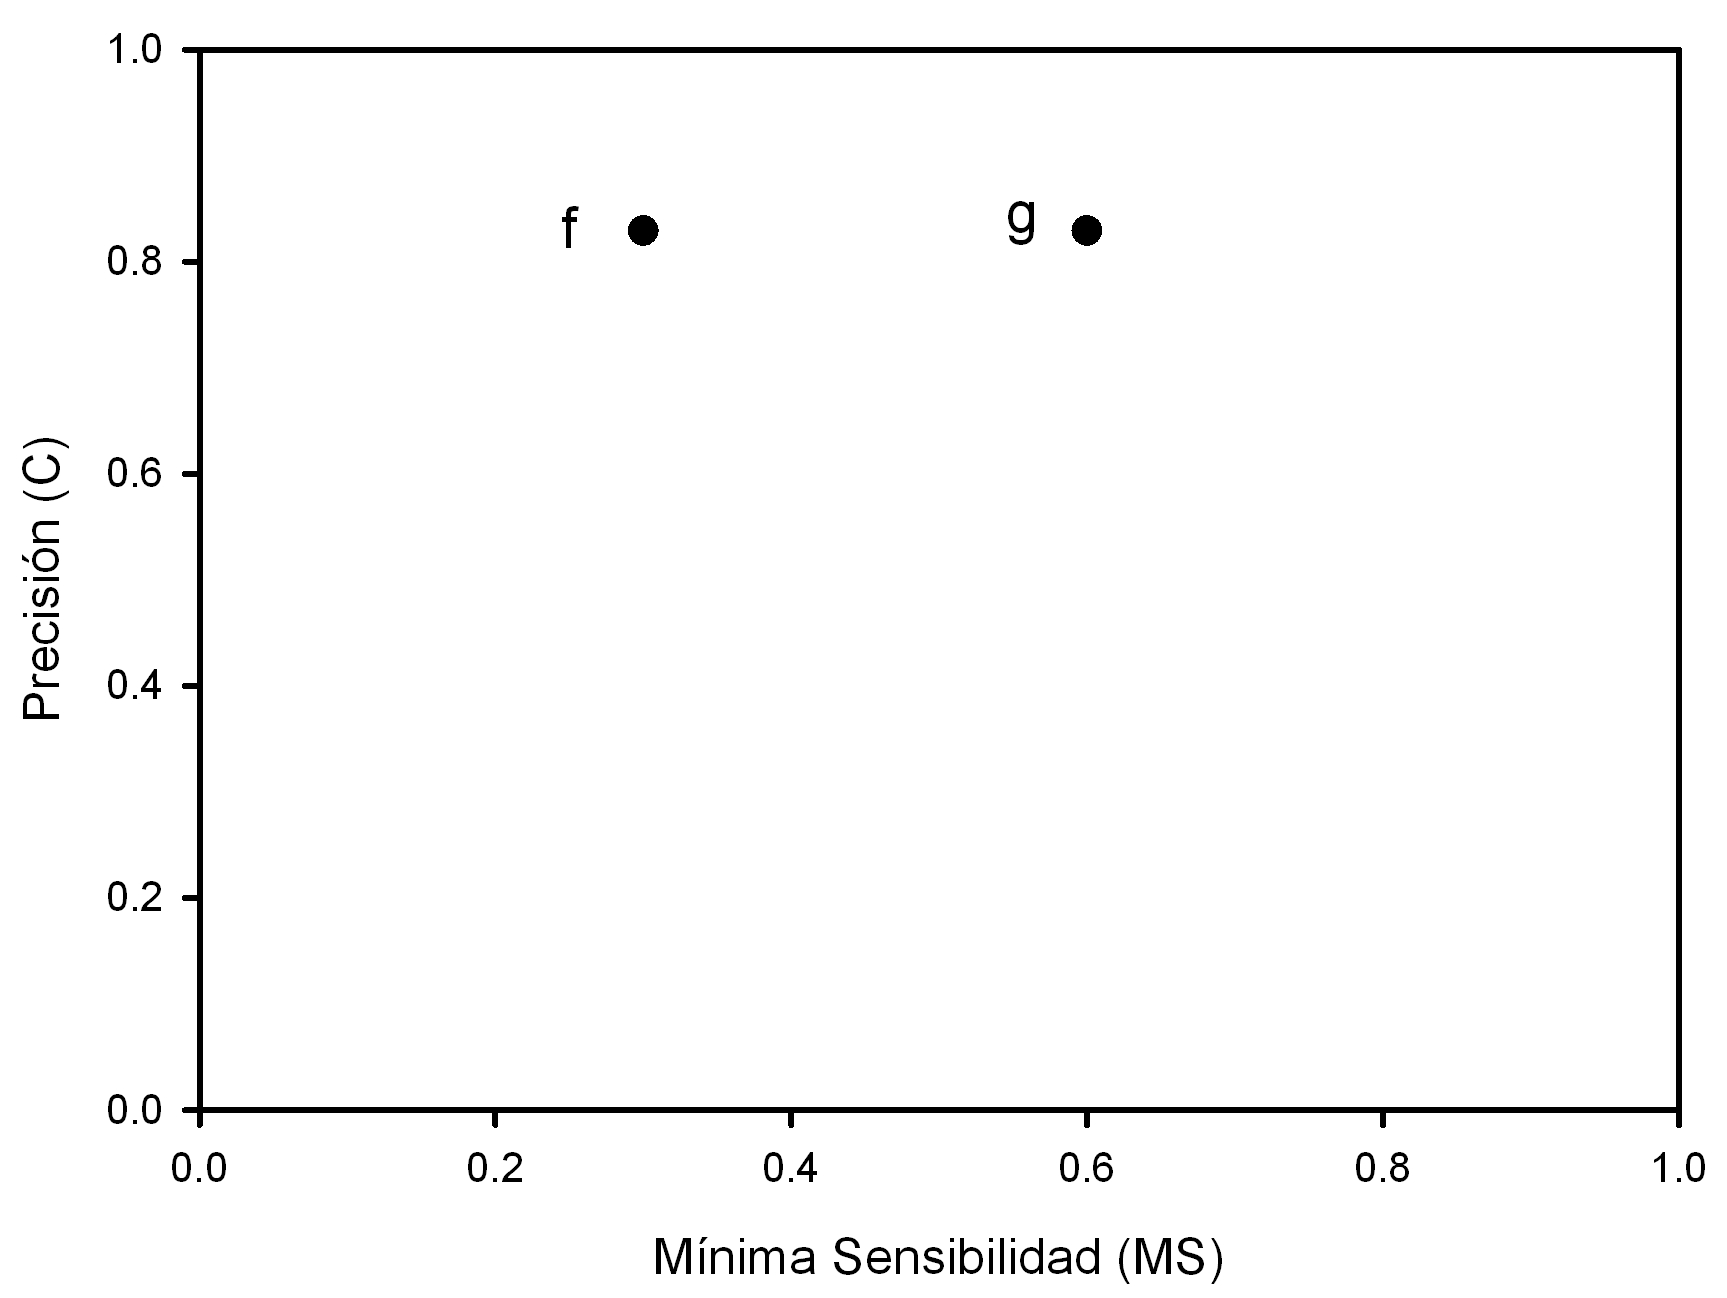
\includegraphics[width=.50
\textwidth]{figuras/articuloMarianoFigure4.jpg}} \\
\subfloat[]{\label{marianoejemplo2}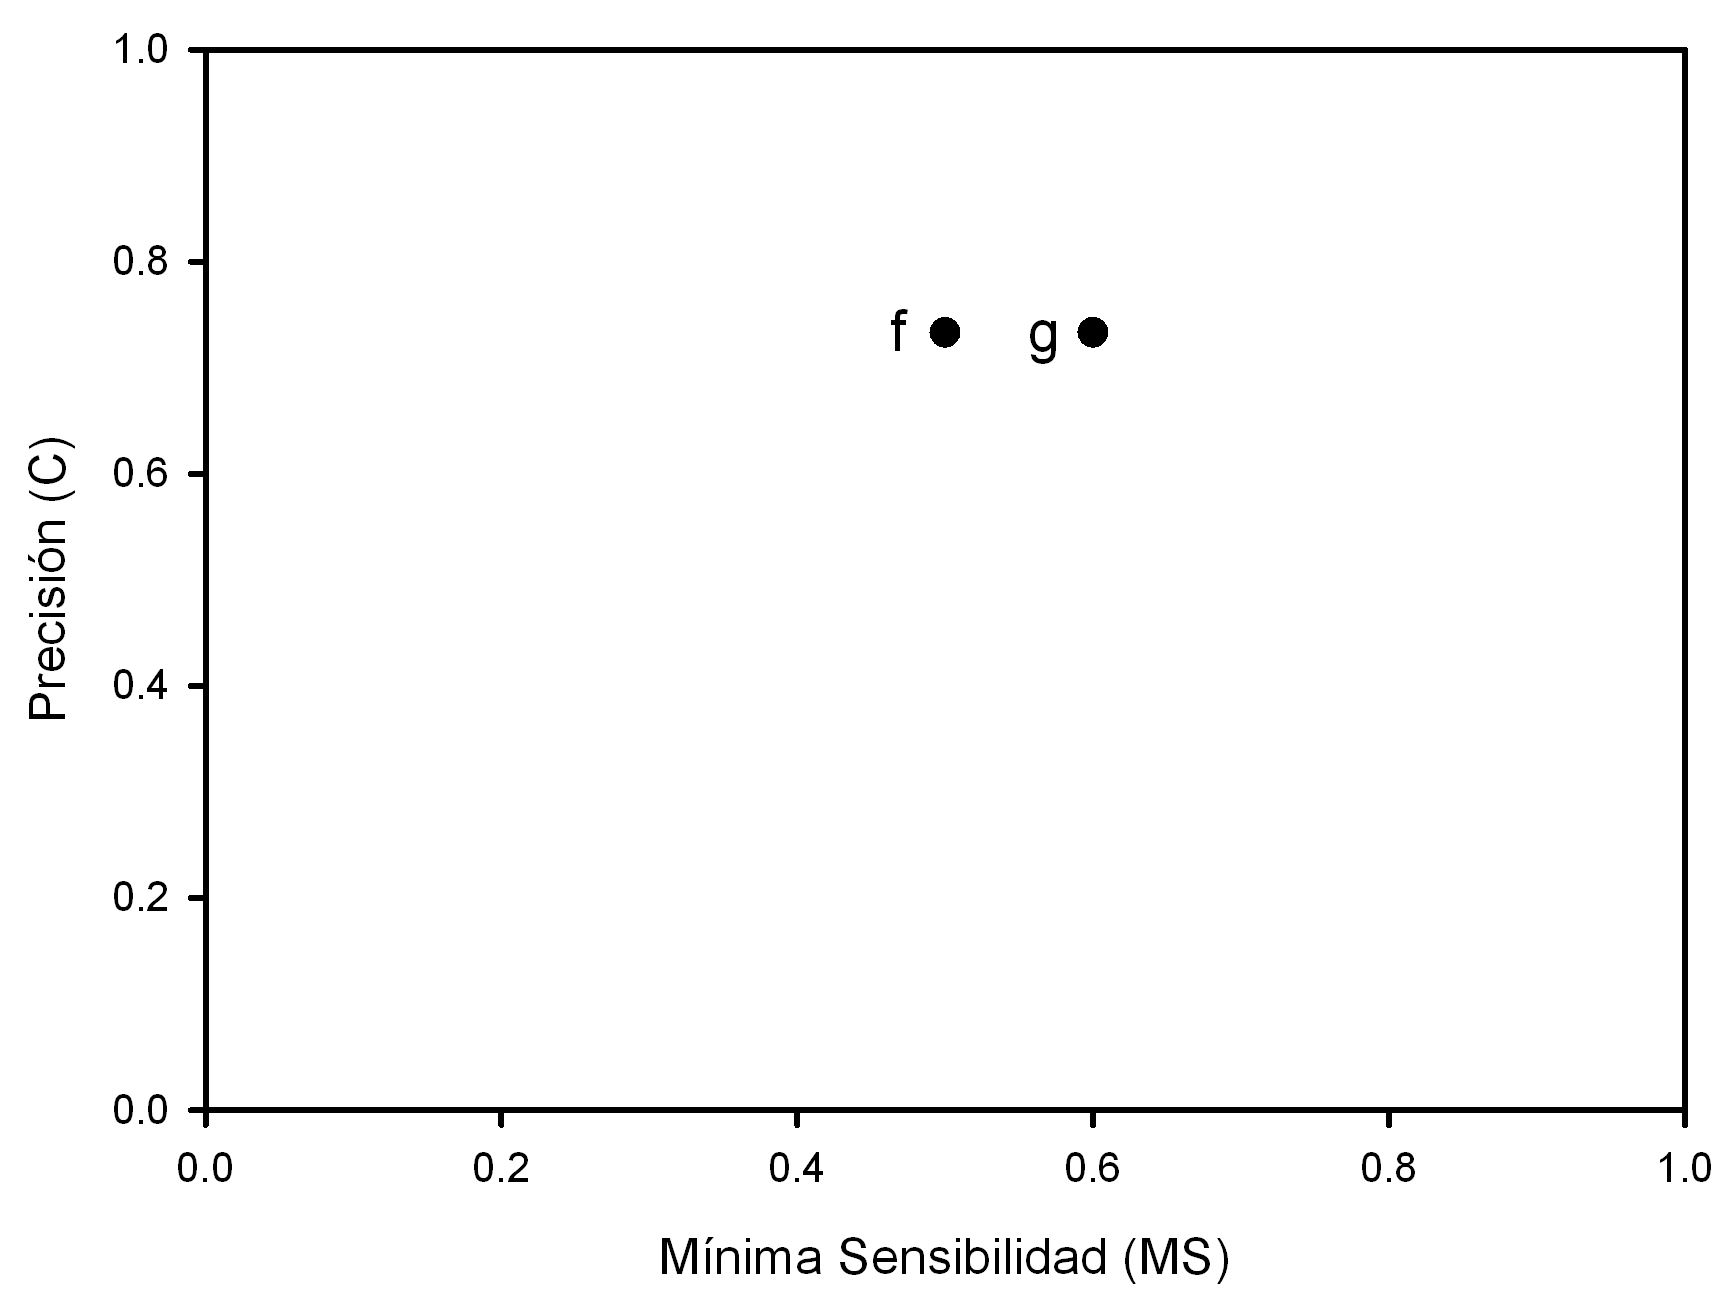
\includegraphics[width=.50
\textwidth]{figuras/articuloMarianoFigure3.jpg}}
\subfloat[]{\label{marianoejemplo4}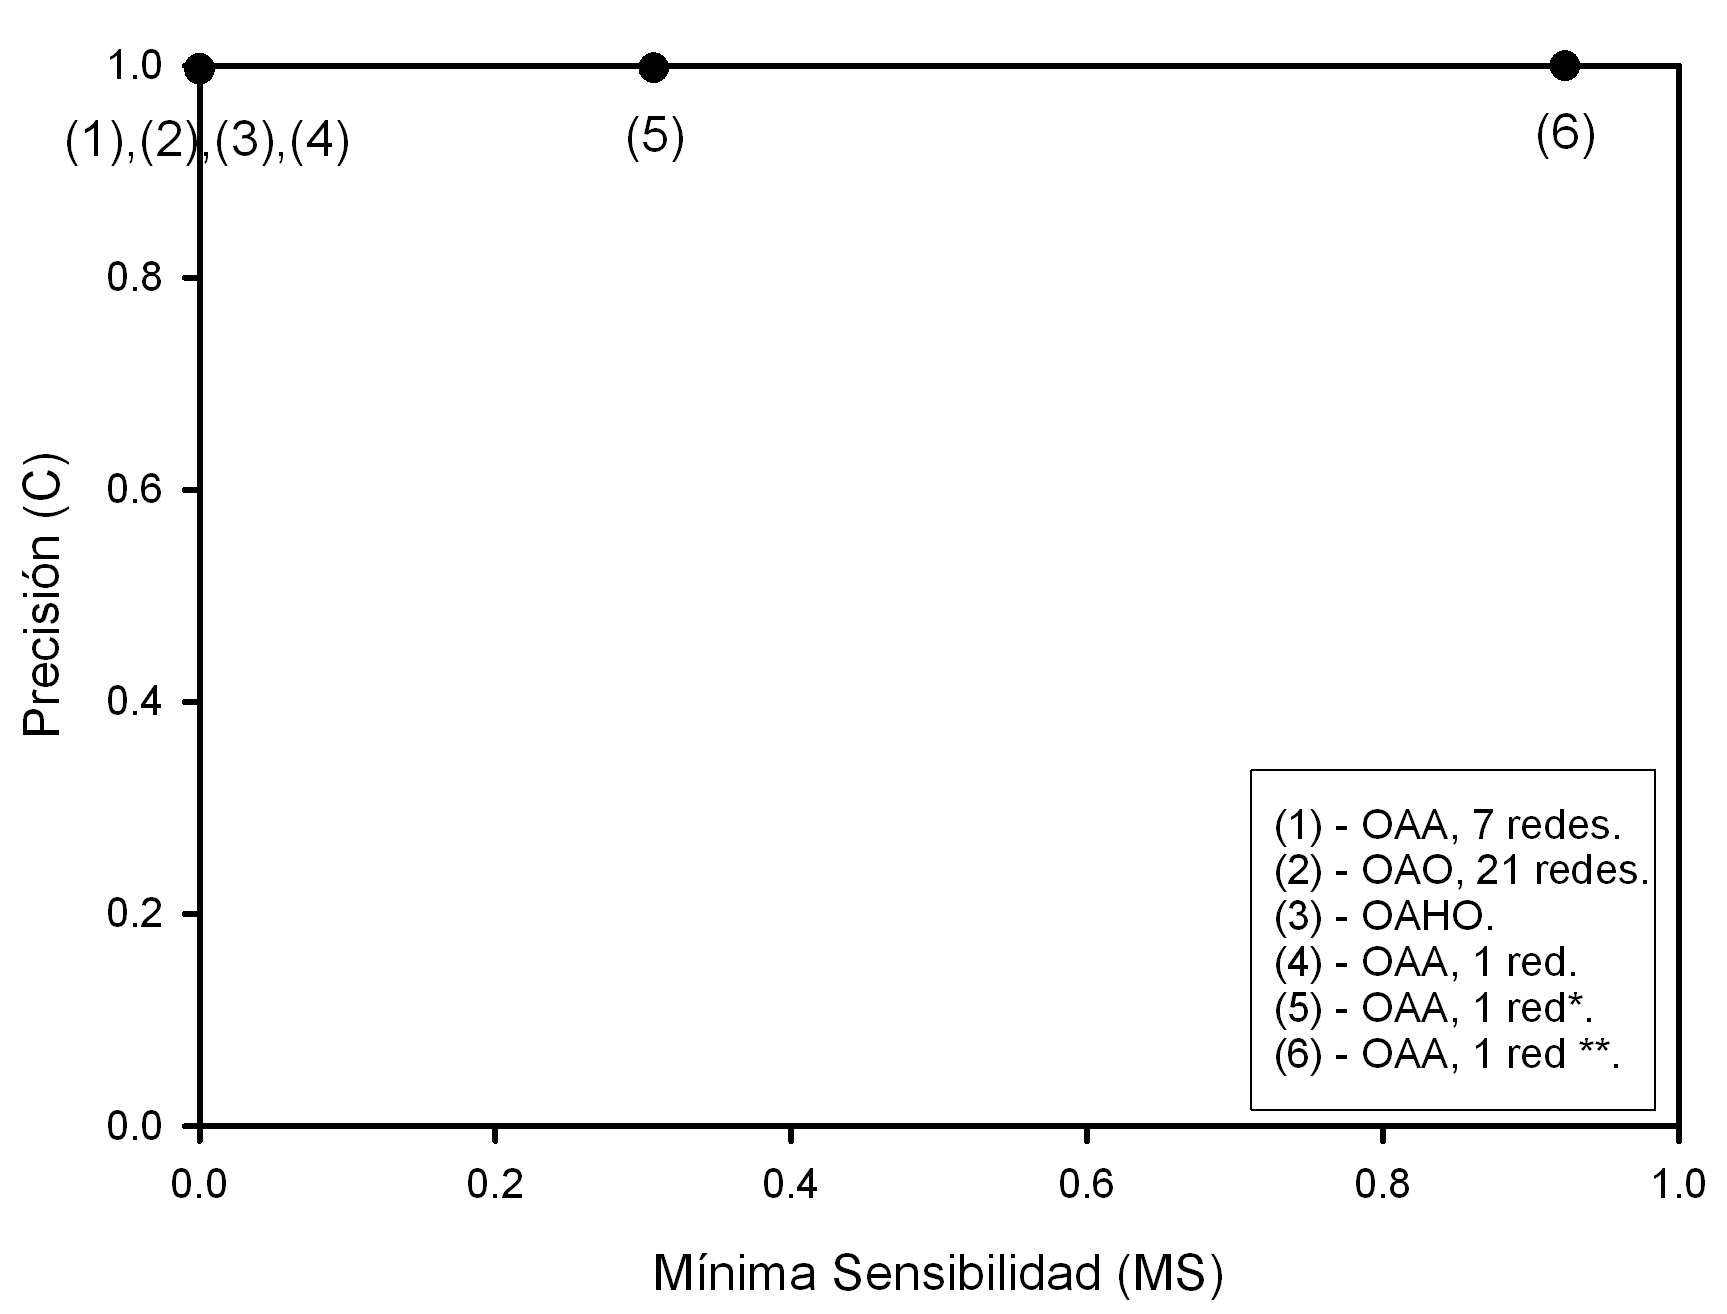
\includegraphics[width=.50
\textwidth]{figuras/articuloMarianoFigure5.jpg}}
\caption{Clasificadores $f$ y $g$ en el plano $(MS,C)$.}
\label{marianofigures}
\end{figure*}

\textbf{Ejemplo 2 (Inadecuación de la macro-media):} Permítanos considerar un problema de
clasificación con cinco clases de tamaño 250, 150, 100, 100 y 10 respectivamente, y las
correspondientes matrices de confusión, $A$ y $B$,  asociadas a dos clasificadores $f$ y
$g$, con los siguientes elementos de la diagonal principal:
\begin{displaymath}
diag(A)=\left( 155,150,99,99,3\right); \quad
diag(B)=\left( 200,150,83,67,6\right),
\end{displaymath}
pudiendo tomar los valores exteriores a la diagonal principal cualquier valor.

Ambos clasificadores tienen la misma $MAVG$. Las sensibilidades para cada clase en el
clasificador $f$ son $\displaystyle S_{1}=0.62, S_{2}=1, S_{3}=0.99, S_{4}=0.99,
S_{5}=0.3$ y las del clasificador $g$ son $\displaystyle S_{1}=0.8, S_{2}=1, S_{3}=0.83,
S_{4}=0.67, S_{5}=0.6$. Así, la macro media de $f$ y $g$ es $\displaystyle \left( 1/5
\cdot \sum_{i=1}^5 S_{i}\right) =0.78$, con lo que no distingue a los clasificadores.

\textbf{Contraejemplo 2:} Los clasificadores del ejemplo 2 tienen la misma $MAVG$
y las precisiones de ambos son $\displaystyle \frac{506}{610}=0.829$, la $MS$ de
$f$ es $MS_{f}=0.3$, mientras que la $MS$ del clasificador $g$ es $\displaystyle
MS_{g}=0.6$, por tanto el clasificador $g$ es mejor que el clasificador $f$. En la
representación gráfica mostrada en la figura \ref{marianoejemplo3} se puede ver como $g$
domina a $f$.

\textbf{Ejemplo 3 (Inadecuación de la media geométrica):} Permítanos considerar un
problema de clasificación con 300 patrones y tres clases de 100, 100 y 100 patrones
respectivamente. Sean $A$ y $B$ las matrices de confusión correspondientes a los
clasificadores $f$ y $g$, de forma que sus diagonales principales vienen dadas por:
\begin{displaymath}
diag(A)= (50,80,90); \quad diag(B)= (60,60,100)
\end{displaymath}
Las sensibilidades para cada clase en el clasificador $f$ son $S_{1}=0.5, S_{2}=0.8,
S_{3}=0.9$ y para el clasificador $g$ son $S_{1}=S_{2}=0.6, S_{3}=1$, y la media
geométrica de los dos es $GM(f)=GM(g)=0.711$.

\textbf{Contraejemplo 3:} Los clasificadores del ejemplo 3 poseen la misma precisión
$C=0.733$. La $MS$ del clasificador $f$ es $MS_{f}=min\left\lbrace
0.5,0.8,0.9\right\rbrace = 0.5$, mientras que la de $g$ es $MS_{g}=min\left\lbrace
0.6,0.6,1\right\rbrace = 0.6$, por tanto podríamos decir que el clasificador $g$ es mejor
que el clasificador $f$ (ver figura \ref{marianoejemplo2}).

\textbf{Ejemplo 4:} Para este ejemplo hemos considerado los resultados obtenidos por
diferentes metodologías en \cite{Ou2007}. Los autores utilizan cuatro sistemas de ANNs con distinto
número de redes para la clasificación de patrones:
un sistema basado en un esquema uno contra uno (\textit{One Against One} OAO), un sistema
uno contra todos (\textit{One Against All}, OAA) para redes binarias, una red neuronal
simple entrenada con un esquema OAA, y un sistema de modelado uno contra el mejor orden
(\textit{One Against Higher Order}, OAHO). Estas metodologías se aplican a dos conjuntos
de datos desbalanceados, \textit{Glass} y \textit{Shuttle}. A partir de la tabla
\ref{tablaEjemplo4}, que se corresponde con la tabla 4 del citado artículo, podemos
representar los clasificadores obtenidos en el plano $(MS,C)$ para el conjunto de datos
\textit{Shuttle} (figura \ref{marianoejemplo4}). Dichos resultados muestran que la
metodología OAA con una red obtiene un clasificador dentro del plano $(MS,C)$ que domina a
los demás y que la precisión no distingue prácticamente entre las 6 metodologías.

\begin{table}[!htb]
\caption{Mínima sensibilidad, $MS$, y precisión, $C$, para los clasificadores en el
conjunto de datos Shuttle.}
\label{tablaEjemplo4}
\centering
\begin{tabular}{p{4cm}p{3.2cm}p{2.8cm}} \hline
\rowcolor[rgb]{0.70,0.85,1}\textbf{Metodología} & $\mathbf{MS}$ & $\mathbf{C}$\\ \hline
\rowcolor[rgb]{0.86,0.94,1}OAA, 7 redes & 0 & 0.9963\\
\rowcolor[rgb]{0.86,0.94,1}OAO, 21 redes & 0 & 0.9969\\
\rowcolor[rgb]{0.86,0.94,1}OAHO & 0.076 & 0.9969\\
\rowcolor[rgb]{0.86,0.94,1}OAA, 1 red & 0 & 0.9963\\
\rowcolor[rgb]{0.86,0.94,1}OAA, 1 red * & 0.307 & 0.9977\\
\rowcolor[rgb]{0.86,0.94,1}OAA, 1red ** & 0.923 & 0.9977 \\ \hline
\multicolumn{3}{l}{* Con duplicación previa de los datos de la clase minoritaria.} \\
\multicolumn{3}{l}{** Entrenamiento con datos de la clase minoritaria e incremento}
\\
\multicolumn{3}{l}{de la capacidad de la red para entrenamiento posterior con datos} \\
\multicolumn{3}{l}{dinámicos.}
\end{tabular}
\end{table}

\section{Propiedades de las medidas $(MS,C)$}\label{propiedades}
Previo a definir las propiedades de las medidas $(MS,C)$, es necesario establecer cuál
es la relación entre ambas:

Consideremos un problema de clasificación con $Q$ clases, siendo $C$ y $MS$ las
medidas asociadas a un clasificador $g$, y $p^*$ la mínima de las frecuencias relativas
de cada clase calculadas ''a priori``. De esta forma, podemos representar los valores
de $MS$ y $C$ en un eje de coordenadas, concretamente $MS$ en el eje $X$ y $C$ el eje $Y$,
de manera que se puede visualizar fácilmente el rendimiento de un clasificador, sin tener
en cuenta el número de clases	que tenga el problema.

Un punto en el plano $\left(MS,C\right)$ domina a otro si tiene un mayor valor de $C$ e
igual o mayor valor de $MS$, o si tiene mayor valor de $MS$ y mayor o igual de $C$.
Idealmente, a partir de la desigualdad \ref{desigualdad3}, cada clasificador se puede
representar como
un punto en la región blanca de la figura \ref{regionFactible}, de forma que el área
exterior al triángulo se marca como región no factible. El área interior al triángulo
puede ser factible a priori, dependiendo del clasificador y de la dificultad del problema;
así el clasificador óptimo $\left(MS=1,C=1\right)$ no es posible o factible para todos los
problemas y clasificadores, especialmente para problemas con elementos estocásticos. Por
esta razón es mejor decir que un clasificador no puede estar localizado en el área
marcada como región no factible. Además, puntos situados en el eje vertical
corresponderían a clasificadores que no son capaces de predecir correctamente ningún
elemento de una clase determinada. Hay que hacer notar que es posible encontrar algunos
clasificadores con un valor de $C$ alto, particularmente en problemas con valores pequeños
de $p^*$ o incluso $0$ (problemas no balanceados), y sin embargo con un valor de $MS$
bajo. Para valores de $C$ menores que $(1-p^*)$, el rango de posibles valores de $MS$
aumenta con respecto al valor de $C$, sin embargo cuando $C$ es mayor que $(1-p^*)$ el
rango de posibles valores de $MS$ disminuye cuando $C$ aumenta.

\begin{figure}[htb]
\centering
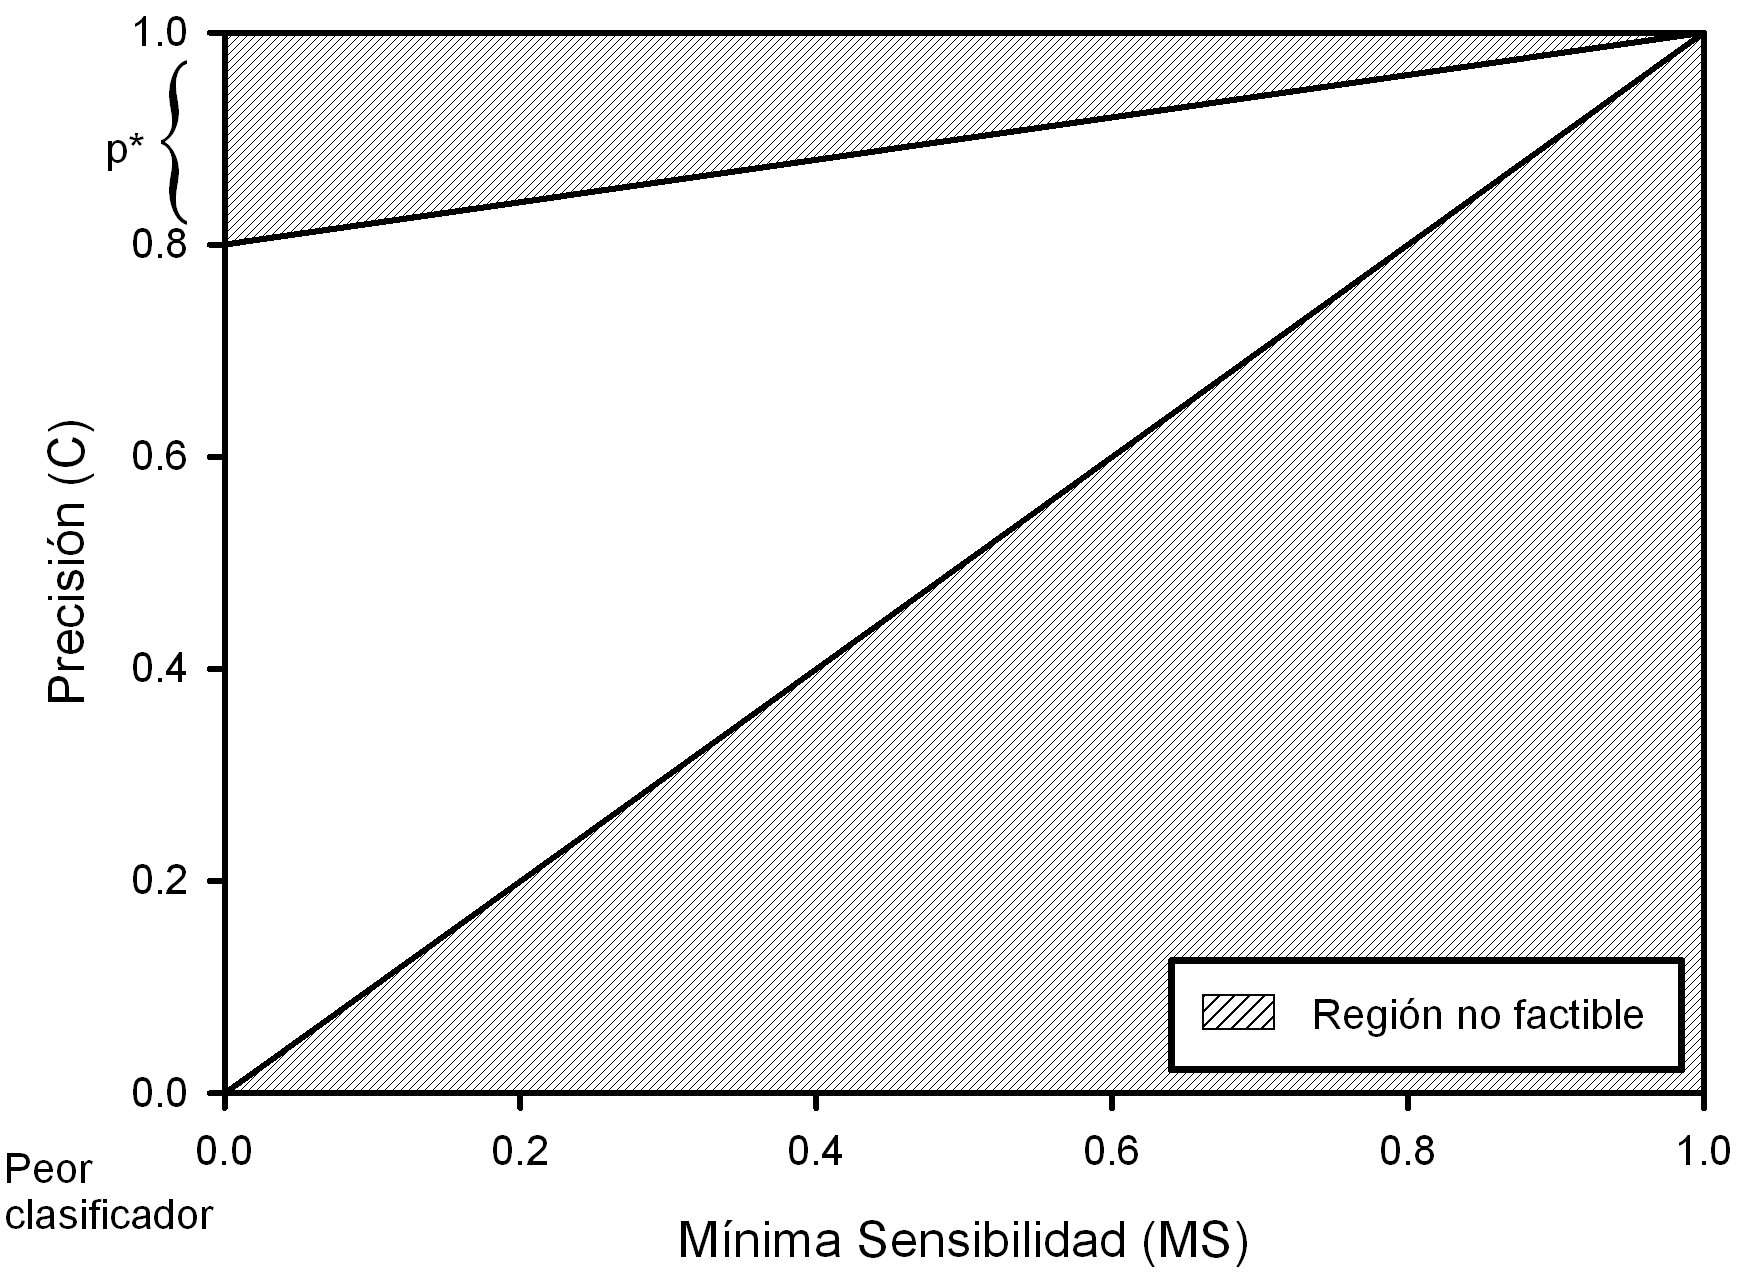
\includegraphics[keepaspectratio,width=11cm]{figuras/regionFactible.jpg}
\caption{Región no factible en el plano $\left(MS,C\right)$ para un
problema de clasificación con $p^*=0.2$.}
\label{regionFactible}
\end{figure}

Obsérvese que un incremento en $C$, no implica necesariamente un incremento
en $MS$. Recíprocamente, un incremento en la $MS$ no significa un
incremento en $C$. Por otro lado, es necesario decir que para un determinado
valor de $C$, un clasificador será mejor cuando se acerque a un punto lo más cercano
posible a la diagonal de la figura \ref{regionFactible} (tanto $C$ como $MS$ toman valores en el
intervalo
$\left[0,1\right]$). Si se utilizan MOEAs como metodología para
la obtención de clasificadores, al comienzo del proceso evolutivo, $MS$ y $C$ pueden ser
cooperativas, e incluso estar lineal y correladas positivamente, pero después de un
determinado número de generaciones, estos objetivos
llegan a ser competitivos, es decir, una mejora en uno de ellos, en general supone un
empeoramiento en el otro. En la Figura \ref{CvsS} se puede ver un ejemplo en el que $MS$ y
$C$ son, en general, objetivos en conflicto, ya que para aumentar el valor de $MS$ en el
clasificador $g_{1}$ es necesario ''perder`` la clasificación de algunos patrones, de
manera que $C$ disminuye en $g_{2}$.
\begin{figure}[htb]
\centering
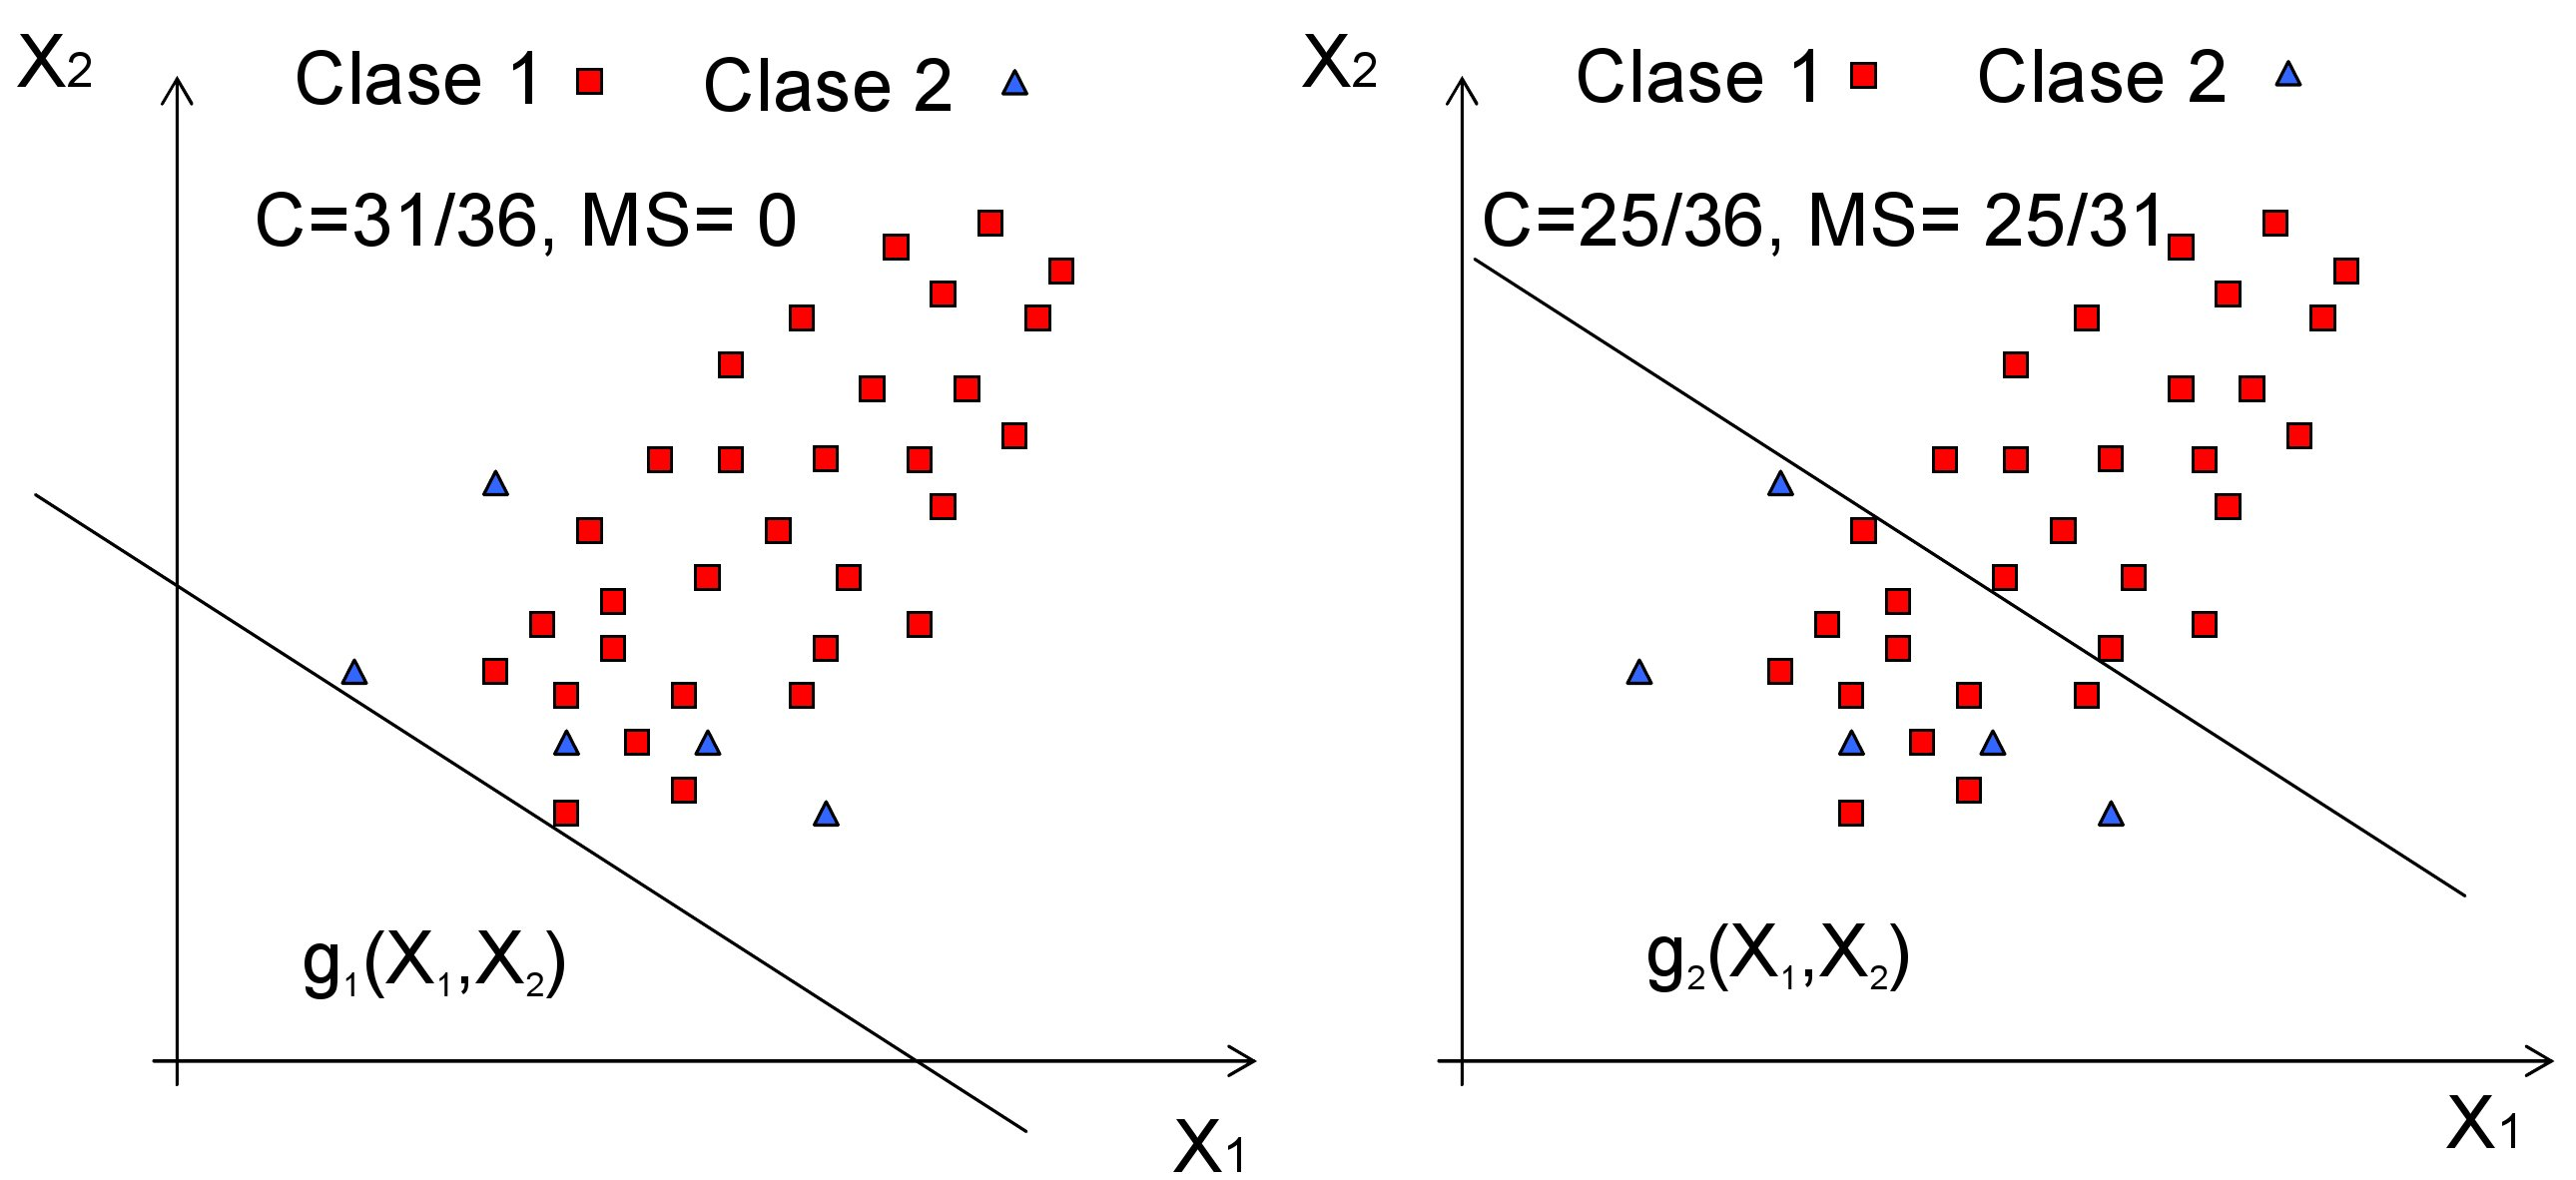
\includegraphics[keepaspectratio,width=12.5cm]{figuras/CvsS.jpg}
\caption{Ejemplo gráfico para describir $MS$ y $C$ como objetivos en
conflicto.}
\label{CvsS}
\end{figure}

A continuación se muestran las propiedades de las medidas $(MS,C)$ como medidas de rendimiento de
un clasificador:
\begin{description}
\item[\textbf{Proposición 1.}] Consideremos de nuevo un problema de clasificación con $Q$
clases, y $J$ la clase con la mínima probabilidad de pertenencia o $p^{*}$, es
decir, $p^{*}=\frac{n_{J\circ}}{N}$, siendo $n_{J\circ}$ el tamaño de la clase
más pequeña y $N$ el tamaño del conjunto de datos. Esta consideración da lugar a la
siguiente desigualdad $MS\leq C\leq 1- \left(1-MS \right) p^{*}$.
\item[\textbf{Demostración.}] Comenzamos demostrando el límite superior de la
inecuación. Teniendo en cuenta
las definiciones de $C$ y $MS$, y que $\displaystyle \sum_{i=1}^Q n_{i\circ}=N$ se puede
comprobar que:
\begin{eqnarray}\label{desigualdad1}
C=\sum_{i=1}^Q \frac{n_{ii}}{n_{i\circ}}\frac{n_{i\circ}}{N}=\sum_{i=1}^Q
S_{i}\frac{n_{i\circ}}{N}=;MS\frac{n_{J\circ}}{N}+\sum_{i\neq
J}S_{i}\frac{n_{i\circ}}{N}\leq\\
\leq MS\frac{n_{J\circ}}{N}+\sum_{i\neq
J}\frac{n_{i\circ}}{N}=MS\frac{n_{J\circ}}{N}+1-\frac{n_{J\circ}}{N}
=1-\left(1-MS\right)\frac{n_{J\circ}}{N}
\nonumber
\end{eqnarray}
Por otro lado, el límite inferior se obtiene de la siguiente forma:
\begin{equation}\label{desigualdad2}
C=\frac{1}{N}\sum_{i=1}^Q n_{ii}=\sum_{i=1}^Q
\frac{n_{ii}}{n_{i\circ}}\frac{n_{i\circ}}{N}=\sum_{i=1}^Q S_{i}\frac{n_{i\circ}}{N}\geq
MS\sum_{i=1}^Q\frac{n_{i\circ}}{N}=MS
\end{equation}
uniendo (\ref{desigualdad1}) y (\ref{desigualdad2}) se puede concluir que
\begin{equation}\label{desigualdad3}
MS\leq C\leq	1-\left(1-MS\right) p^{*}
\end{equation}
% La relación entre $C$ y $MS$ se puede ver en la figura \ref{regionFactible}, de la
% cual se hablará más detalladamente en la sección \ref{seccionfactible}.
\item[\textbf{Proposición 2.}] Sea un problema de clasificación con $Q$ clases y $p^*$ la
mínima de las frecuencias relativas de clase calculadas ''a priori``. Cada punto $(MS,C)$
perteneciente al subconjunto
\begin{displaymath}
		F=\left\lbrace 	(MS,C):0\leq MS\leq 1, MS\leq C\leq 1-p^*+(MS)p^*\right\rbrace
\end{displaymath}
corresponde al menos a un clasificador $g$. Así, el subconjunto completo $F$ es
factible.
\item[\textbf{Demostración.}] Para probar que el subconjunto $F$ es factible,
probaremos que cada punto de dicho subconjunto se puede obtener a partir de una matriz de
confusión. Sea $\left( MS_{0},C_{0}\right)$ un punto en $F$, la demostración se basa en
la construcción de una matriz de confusión con $MS=MS_{0}$ y $C=C_{0}$ para ese punto.
Definamos la función continua y lineal $f:\left[ MS_{0},1\right]
\rightarrow\mathbb{R}$ como:
\begin{displaymath}
f(MS)=(MS_{0})p^*+MS(1-p^*)
\end{displaymath}
la cual satisface
\begin{displaymath}
f(MS_{0})=MS_{0}\leq C_{0}, f(1)=1-p^*+(MS_{0})p^*\geq C_{0}
\end{displaymath}

La continuidad de la función $f$ implica que existe un valor $MS^*\in \left[
MS_{0},1\right]$ de manera que $f(S^*)=C_{0}$. Definamos la siguiente matriz de
confusión:
\setlength{\arraycolsep}{0.75pt}
\renewcommand{\arraystretch}{1.75}
\scriptsize
\[\begin{array}{ccccccccc}
Clase &  & 1 & 2 & \cdots & Q-1 & Q &  &  \\
1 & \multirow{5}{*}{$\left(
\begin{array}{c}
\\
\\
\\
\\
\\
\end{array}\right.$} & (MS_{0})p^* &
(1-MS_{0})p^* & \cdots & \cdots & 0 & \multirow{5}{*}{$\left.
\begin{array}{c}
\\
\\
\\
\\
\\
\end{array}\right)$} & p^* \\
2 &  & \frac{(1-S^*)(1-p^*)}{Q-1} & \frac{S^*(1-p^*)}{Q-1} & \cdots & \cdots & 0 &  &
\frac{1-p^*}{Q-1}\\
\cdots &  & \cdots & \cdots & \cdots & \cdots & \cdots &  & \cdots\\
Q-1 &  & 0 & 0 & \frac{(1-S^*)(1-p^*)}{Q-1} & \frac{S^*(1-p^*)}{Q-1} & 0 &  & \cdots\\
Q &  & 0 & 0 & \cdots & \frac{(1-S^*)(1-p^*)}{Q-1} & \frac{S^*(1-p^*)}{Q-1} &  &
\frac{1-p^*}{Q-1}
\end{array}\]
% Reestrabelcemos de nuevo los tamaños por defecto
\normalsize
\renewcommand{\arraystretch}{1}
\setlength{\arraycolsep}{1pt}
\newline

Se puede observar que las sensibilidades cumplen lo siguiente:
\begin{displaymath}
S_{1}=S_{0}, S_{2}=...=S_{Q}=\frac{S^*(1-p^*)}{Q-1}
\frac{Q-1}{1-p^*}=S^*
\end{displaymath}

Por tanto $\displaystyle
MS=min\left\lbrace MS_{0},S^*\right\rbrace=MS_{0}$, ya que $\displaystyle S^*\in\left[
MS_{0},1\right]$. Por otra parte, se verifica que la precisión, $C$, asociada a la matriz
es:
\begin{displaymath}
C=MS_{0}p^*+(Q-1)S^* \frac{1-p^*}{Q-1}=f(S^*)=C_{0}
\end{displaymath}
Finalmente, a partir de la condición $\displaystyle p^*\leq \frac{1}{Q}$ obtenemos que
\begin{displaymath}
p^*Q\leq1 \Longrightarrow p^*Q-p^*\leq 1-p^*\Longrightarrow p^*\leq \frac{1-p^*}{Q-1}
\end{displaymath}
y podemos concluir que la mínima probabilidad de las columnas es $p^*$.
\item[\textbf{Proposición 3.}] El área $A$ del conjunto factible $F$ (región dibujada en
blanco en la figura \ref{regionFactible}) verifica que $\displaystyle A= \frac{1-p^*}{2}$,
donde $p^*$
es la mínima de las frecuencias relativas de cada clase.
\item[\textbf{Demostración.}] La demostración es inmediata a partir de la Proposición 2.
Cuando el número de clases aumenta o el problema es altamente desbalanceado, el valor de
$\displaystyle p^*\leq \frac{1}{Q}$ disminuye en ambos casos. Por tanto una consecuencia
de la Proposición 3 es que, el área de $F$ aumenta cuando el nivel de desbalanceo o el
número de clases aumenta. Un análisis similar prueba que el valor mínimo del área se
alcanza cuando el problema es totalmente balanceado, es decir, $\displaystyle p^*=
\frac{1}{Q}$. En consecuencia, en problemas no balanceados, la línea que define el borde
superior del conjunto en el plano $(MS,C)$
tiende a ser horizontal, y el rango de valores de $MS$ será mayor incluso para valores
altos de $C$. En este caso, el valor de $C$ como medida única de un clasificador
multiclase es insuficiente, ya que esconde muchas posibilidades diferentes para $MS$.
Estos comentarios muestran que las medidas $(MS,C)$ pueden ser especialmente ventajosas
en problemas con cierto desbalanceo o cuando el número de clases es alto, confirmando
que, por si sola, la medida $C$ es inadecuada en estas situaciones.

Finalmente, analizamos la relación existente entre las medidas $(MS,C)$ y las curvas
ROC en problemas binarios. Los siguientes resultados establecen la relación
entre los dos espacios en un problema de clasificación binario, probando que no hay
equivalencia entre ellos. En este sentido las medidas $(MS,C)$ constituyen un punto de vista
complementario a las curvas ROC en problemas binarios.
\item[\textbf{Proposición 4.}] Sea $Q=2$ el número de clases y $q$ la probabilidad ''a
priori`` de que un patrón pertenezca a la primera clase. Entonces cada punto
$(TPR_{0},FPR_{0})$ en el plano \textit{ROC} determina un único punto factible
$(MS_{0},C_{0})$ en el plano $(MS,C)$ definido por:
\begin{displaymath}
MS_{0}	=min\left\lbrace TPR_{0}, 1-FPR_{0}\right\rbrace \qquad
C_{0}=TPR_{0}q+(1-FPR_{0})(1-q)
\end{displaymath}
Inversamente, cada punto $(MS_{0},C_{0})$ de $F$, determina dos puntos en el plano
\textit{ROC} dado por:
\begin{align}
	FPR_{1}&=\frac{1-C_{0}-(1-MS_{0})q}{1-q},\qquad TPR_{1}=MS_{0} \nonumber \\
	FPR_{2}&=1-MS_{0}, \qquad TPR_{2}=\frac{C_{0}-MS_{0}(1-q)}{q} \nonumber
\end{align}
\item[\textbf{Demostración.}] Sea $\displaystyle (TPR_{0},FPR_{0})$ un punto en el
plano ROC, supongamos que la matriz de confusión está dada por $\left( \begin{array}{cc}
n_{11} & n_{12}\\
n_{21} & n_{22}
\end{array}\right) $, y sea $N$ el número de patrones. Recordando la definición de
MS, tenemos que
\begin{equation}\label{p4-1}
S_{0}=min\left\lbrace TPR_{0}, 1-FPR_{0}\right\rbrace
\end{equation}
Por otro lado, la precisión $C_{0}$ es $\displaystyle \frac{n_{11}}{N}+\frac{n_{22}}{N}$.
Teniendo
en cuenta que $\displaystyle TPR_{0}=\frac{n_{11}}{n_{1\circ}}$ y
$FPR_{0}=\frac{n_{21}}{n_{2\circ}}$, donde $n_{1\circ}=n_{11}+n_{12}$ y
$n_{2\circ}=n_{21}+n_{22}$ son
el número de patrones en la primera y segunda clase respectivamente, y que $q$ es la
probabilidad "a priori" de la primera clase, tenemos
\begin{equation}\label{p4-2}
\begin{split}
C_{0}&=\frac{n_{11}}{N}+\frac{n_{22}}{N}=\frac{n_{11}}{n_{1\circ}}\frac{n_{1\circ}}{N}
+\frac{n_ {22}}
{n_{2\circ}}\frac{n_{2\circ}}{N}= \\
&=(TPR_{0})q+(TPR_{0})(1-q)=(TPR_{0})q+(1-FPR_{0})(1-q)
\end{split}
\end{equation}
Inversamente, si $(MS,C)$ es un punto factible, a partir de las ecuaciones \ref{p4-1} y
\ref{p4-2} previamente establecidas se tiene que
\begin{align}
FPR_{1}&=\frac{1-C_{0}-(1-S_{0})q}{1-q},\qquad TPR_{1}=S_{0} \nonumber \\
FPR_{2}&=1-S_{0}, \qquad TPR_{2}=\frac{C_{0}-S_{0}(1-q)}{q} \nonumber
\end{align}
dependen estos puntos de la clase en la que la sensibilidad alcance el valor más bajo.
Obsérvese que $0\leq TPR_{0},FPR_{0}\leq1$.
A partir de estos resultados podemos hacer las siguientes observaciones:
\begin{enumerate}
	\item Es fácil probar que
	\begin{displaymath}
	FPR_{2}=FPR_{1}+\frac{C-SM}{1-q}, \qquad TPR_{2}=TPR_{1}+\frac{C-MS}{q}
	\end{displaymath}
	siendo la pendiente del segmento que une los puntos ROC asociados el
	$\displaystyle \left(\frac {1-q}{1}\right) $ por ciento entre las probabilidades ''a
priori``,
	independientemente del punto $(MS_{0},C_{0})$ considerado. Como $\displaystyle
	\left( \frac{1-q}{1}>0\right)$, ningún punto domina a los demás.
	\item Los puntos obtenidos en el plano ROC son iguales, si y solo si, $MS=C$.
	Es decir, los puntos en la diagonal del plano $(MS,C)$ determinan solamente un punto en
el
	plano ROC.
\end{enumerate}
\end{description}

\section{Problemas no balanceados y/o con gran número de clases}\label{balanceados}
\noindent Como ya hemos comentado en la sección anterior, cuando el número de clases
aumenta, o cuando existe un problema altamente
desbalanceado, el valor de $\displaystyle p^*=\frac{n_{\circ j}}{N}\leq \frac{1}{Q}$ disminuye, y la
línea
del borde superior de la región factible, dentro del plano $\left(MS,C\right)$, tiende a
ser horizontal, es decir, a tomar el valor $C=1$, de manera que el rango de valores de
$MS$ será más amplio cuando $C$ tome valores altos. En este tipo de problemas
\cite{Ho2002,Murphey2004} es difícil
mantener un nivel de precisión alto en cada clase,	debido a la dificultad en el
aprendizaje a partir de clases con pocos patrones, que puede conllevar una disminución
del valor de $C$ en el conjunto de generalización.

De forma general, la solución aportada al tratamiento de problemas no balanceados se
puede dividir en aproximaciones a nivel de datos y aproximaciones a nivel de algoritmo
\cite{He2009,Sun2009}.

\begin{itemize}
\item A nivel de datos, la solución es rebalancear la distribución por clase mediante
técnicas
de remuestreo, ya sea quitando patrones de la clase mayoritaria o incluyéndolos en la
minoritaria, o incluso una combinación de las dos \cite{Kubat97,Chawla2002}. Estos métodos
conllevan desventajas:
\begin{enumerate}
\item La distribución óptima por clase de un conjunto de entrenamiento es usualmente
desconocida.
\item Una estrategia de remuestreo poco efectiva
puede ocasionar riesgos de pérdida de información sobre las clases mayoritarias en caso de
hacer un muestreo eliminando patrones, o sobre las clases minoritarias, en caso de hacer
un muestreo aumentando el numero de patrones, pudiendo en este último caso ocasionar un
sobreajuste o sobreaprendizaje de los datos.
\item En la mayoría de los casos existe un inevitable coste extra relacionado con el
análisis y procesamiento de los datos.
\end{enumerate}
\item A nivel algorítmico, lo que se hace es adaptar el aprendizaje del algoritmo
para que influya sobre la clase minoritaria \cite{Jankowski2001b}. En \cite{Fernandez2009}
y \cite{Fernandez2009a} se pretende que dos EAs para ANNs vayan
nivelando el porcentaje de buena clasificación en cada una de las clases de un
problema determinado, o al menos dejarlas de la manera más equilibrada posible, usando
respectivamente $MS$ y el coeficiente de variación de las sensibilidades de
todas las clases. En \cite{Martinez-Estudillo2008} este objetivo se aborda utilizando un
algoritmo en dos etapas, optimizando $C$ en la primera etapa, y en la segunda optimizando
una función definida a partir de $C$ y $MS$, que geométricamente corresponde al área de un
recinto definido por el clasificador en la región factible de la figura
\ref{regionFactibleAreaEA}, donde dicha área viene definida por:
\begin{displaymath}
A(MS,C)=(1-MS)(1-C)-\frac{1}{2}\left[ (1-C)^2-p^*(1-MS)^2\right]
\end{displaymath}
\end{itemize}

La mayoría de nuevos métodos que se describen en esta tesis doctoral para la obtención de
clasificadores usando las medidas $(MS,C)$ son métodos a nivel de algoritmo, y bajo este
punto
de vista, $MS$ y $C$ pueden ser ventajosas como medidas de precisión en problemas no
balanceados y/o con un número de clases elevado.
\newpage

\begin{figure}[!htp]
\centering
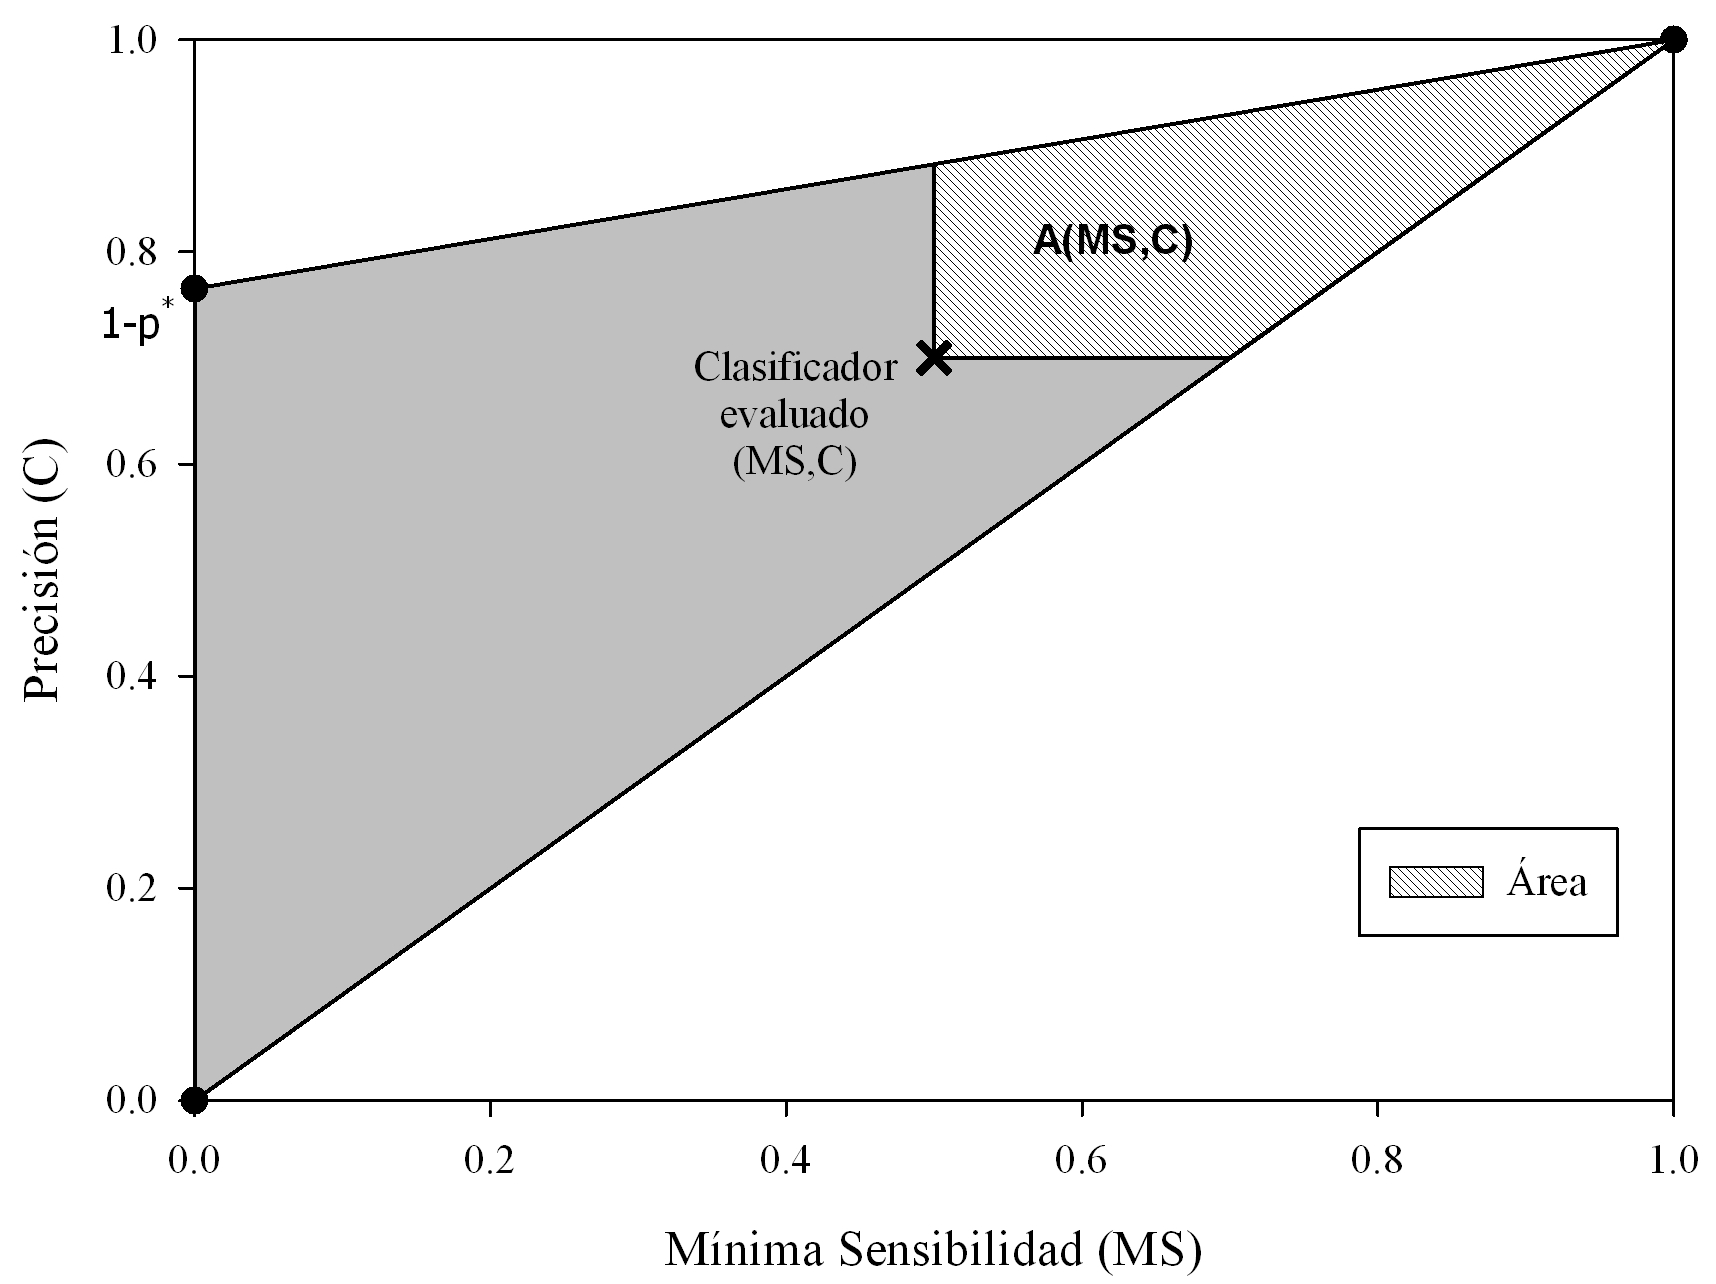
\includegraphics[keepaspectratio,width=9cm]{figuras/EA.jpg}
\caption{Área sobre un clasificador evaluado, función $A(MS,C)$.}
\label{regionFactibleAreaEA}
\end{figure}
\paginavaciacompleta